\documentclass[12pt,oneside]{report}
\usepackage[utf8]{inputenc}
\usepackage{graphicx}
\usepackage{caption}
\usepackage{subcaption}
\usepackage[a4paper,width=150mm,top=25mm,bottom=25mm,bindingoffset=6mm]{geometry}
\usepackage{fancyhdr}
\usepackage[italian]{babel}
\pagestyle{fancy}
\usepackage{biblatex}
\addbibresource{references.bib}
\usepackage{comment}
\usepackage{amsfonts}
\usepackage{tcolorbox}
\usepackage{amsmath}
\usepackage{wrapfig}
\usepackage{tabularx}
\usepackage{csquotes}
\usepackage{adjustbox}
\usepackage{graphicx}
\usepackage{makecell}
\usepackage{footnote}
\usepackage{lscape}
\usepackage{graphicx}
\graphicspath{{figures/}}
\usepackage{array}
\usepackage{threeparttable}
\usepackage{rotating}
\usepackage[titletoc]{appendix}
\DeclareMathOperator*{\argmax}{arg\,max}
\DeclareMathOperator*{\argmin}{arg\,min}
%\usepackage{afterpage}
\usepackage{relsize}
\usepackage{listings}


\newcommand{\newblanckpage}{
    \newpage
    \thispagestyle{plain} % empty
    \mbox{}
}

	
\newcommand{\indep}{\perp \!\!\! \perp}

\begin{document}
\newgeometry{margin=1in}
\begin{titlepage}
    \vspace*{1 cm}
    \begin{center}
         {\LARGE \textbf{Formulario Probabilità e Statistica}\\}
        \vspace{2 cm}
        \textsc{Università Ca' Foscari di Venezia}\\
        Dipartimento di scienze ambientali, informatica e statistica\\
        \vspace{0.2 cm}
        \begin{figure}[h!]
        	\centering
        	
\includegraphics[width=0.6\textwidth]{logo} 
        \end{figure}
        \vspace{0.0 cm} [CT0111] PROBABILITA' E STATISTICA\\
        %\vspace{0.0 cm} Thesis notes\\
        Anno Accademico 2023 - 2024\\
        \vspace{3.0 cm}
        	
        \begin{flushleft}
        	\begin{tabular}{l l}
        		\textbf{Tutor} & Zuliani Riccardo \\
                \textbf{Contatti} & 875532@stud.unive.it
        	\end{tabular}
        \end{flushleft}
    \end{center}
\end{titlepage}

\restoregeometry


\pagenumbering{roman}

\tableofcontents

%\listoffigures

%\listoftables

\clearpage

\pagenumbering{arabic}

\setcounter{page}{1}

\chapter{Probabilità Elementare}
\begin{itemize}
    \item \textbf{Principio fondamentale del calcolo combinatorio:} \(m_1 \times m_2\)
    \item \textbf{Principio fondamentale generalizzato:} \[\prod_{i+1}^rm_i = m_1 \times ... \times m_r\]
    \item \textbf{Disposizioni con ripetizione:} \[\prod_{i=1}^rn = n^r\]
    \item \textbf{Disposizioni semplici:} \(n \times (n - 1) \times ... \times (n - r + 1)\)
    \item \textbf{Permutazioni:} \(n \times (n - 1) \times (n - 2) \times ... \times 2 \times 1 =: n!\)
    \item \textbf{Combinazioni:} \[\frac{n \times (n - 1) \times ... \times (n - r + 1)}{r!} =: {n \choose r}\]
    \item \textbf{Operazioni sugli eventi e Diagrammi di Venn:}
    \begin{itemize}
        \item Complemento \(A^c = 1 - A\)
        \item Intersezione \(A \cap B\)
        \item Unione \(A \cup B\)
        \item Inclusione \(A \subset B\)
        \item Incopatibilita' \(A \cap B = \emptyset\)
    \end{itemize}
    \item \textbf{Assiomi di probabilità:}
    \begin{itemize}
        \item Positivita' \(0 \leq \mathbb{P}[A] \leq 1\)
        \item Normalizzazione \(\mathbb{P}[\Omega] = 1\)
        \item Additivita': se \(A_i \cap A_j = \emptyset\) allora
        \[\mathbb{P}\Bigg[\bigcup_{n=1}^\infty A_n\Bigg] = \sum_{n=1}^\infty \mathbb{P}[A_n]\]
    \end{itemize}
    \item \textbf{Alcune proprietà della probabilità:}
    \begin{itemize}
        \item \textit{Complementare:} \(\mathbb{P}[\bar{A}] = 1-\mathbb{P}[A]\)
        \item \textit{Evento impossibile:} \(\mathbb{P}[\emptyset] = \mathbb{P}[\bar{\Omega}] = 1-\mathbb{P}[\Omega] = 0\)
        \item \textit{Unione:} \(\mathbb{P}[A \cup B] = \mathbb{P}[A] + \mathbb{P}[B] - \mathbb{P}[A \cap B]\)
        \item \textit{Partizione:} se \(C_1, C_2,...\) sono una partizione
         \[\mathbb{P}\Bigg[\bigcup_{n=1}^\infty C_i\Bigg] = \mathbb{P}[\Omega]=1\]
    \end{itemize}
    \item \textbf{Legge della probabilità totale:} \[\mathbb{P}[A] = \sum_i\mathbb{P}[A \cap C_i]\]
    \item \textbf{Eventi elementari equiprobabil:}
    \[\mathbb{P}[A] = \frac{\text{\# casi favorevoli}}{\text{\# possibili casi}}\]
    \item \textbf{Popolazioni e sottopopolazioni}
    \begin{itemize}
        \item \textit{Soluzione con reinserimento:}
        \[\#\Omega = N^n \quad \#A_k ={n \choose k}m^k(N-m)^{n-k}\]
        \begin{flalign*}\mathbb{P}[A_k] &={n \choose k}m^k(N-m)^{n-k}\frac{1}{N^n}\\
                          &={n \choose k}\Big(\frac{m}{N}\Big)^k\Big(\frac{N-m}{N}\Big)^{n-k}\\
                          &={n \choose k}\Big(\frac{m}{N}\Big)^k\Big(1- \frac{m}{N}\Big)^{n-k}
        \end{flalign*}
        \item \textit{Soluzione senza reinserimento:}
        \[\#\Omega = {N \choose n} \quad \#A_k={m \choose k} {N-m \choose n-k}\]
        \[\mathbb{P}[A_k] = \frac{{m \choose k}{N-m \choose n-k}}{{N \choose n}}\]
    \end{itemize}
    
\end{itemize}
\chapter{Probabilità Condizionata}
\begin{itemize}
    \item \textbf{Probabilità condizionata:}
    \[\mathbb{P}[A|B] = \frac{\mathbb{P}[A \cap B]}{\mathbb{P}[B]} \quad \mathbb{P}[B] > 0\]
    \[\mathbb{P}[\bar{A} | B] = \frac{\mathbb{P}[\bar{A} \cap B]}{\mathbb{P}[B]} = \frac{\mathbb{P}[B] - \mathbb{P}[A \cap B]}{\mathbb{P}[B]} = 1 - \mathbb{P}[A | B]\]
    \item \textbf{Formula delle probabilità composte:}
    \[\mathbb{P}[A_1 \cap A_2 \cap ... \cap A_n] = \mathbb{P}[A_1]\mathbb{P}[A_2 | A_1]\mathbb{P}[A_3|A_1 \cap A_2] ... \mathbb{P}[A_n | A_1 \cap ... \cap A_{n-1}]\]
    \item \textbf{Eventi indipendent:} \(\mathbb{P}[A | B] = \mathbb{P}[A]\)
    \item \textbf{\(n\) eventi (reciprocamente) indipendenti:}
    \[\mathbb{P}[A_{i_1} \cap ... \cap A_{i_k}] = \mathbb{P}[A_{i_1}] ... \mathbb{P}[A_{i_k}]\]
    \item \textbf{Sistema in serie:}
    \[\mathbb{P}[A] = \mathbb{P}\Bigg[ \bigcap_{i=1}^nA_i\Bigg] = \prod_{i=1}^n \mathbb{P}[A_i] = \prod_{i=1}^n(a-p_i)\]
    \item \textbf{Sistema in parallelo:}
    \[\mathbb{P}[B] = 1 - \mathbb{P}[\bar{B}] = 1 - \mathbb{P}\Bigg[\bigcap_{i=1}^n\bar{A}_i\Bigg] = 1- \prod_{i=1}^n\mathbb{P}[\bar{A}_i] = 1-\prod_{i=1}^n p_i\]
    \item \textbf{La legge della probabilità totale:}
    \[\mathbb{P}[A] = \sum_i \mathbb{P}[A \cap C_i] = \sum_i \mathbb{P}[C_i]\mathbb{P}[A|C_i]\]
    \item \textbf{La formula di Bayes:}
    \[\mathbb{P}[C_m|A] = \frac{\mathbb{P}[A|C_m]\mathbb{P}[C_m]}{\sum_i\mathbb{P}[A|C_i]\mathbb{P}[C_i]}\]
\end{itemize}
\chapter{Variabili Casuali}
\begin{tcolorbox}[title=Variabili Casuali]
Una \textbf{variabile aleatoria} o \textbf{casuale} \(X\) è una funzione che assume valori numerici determinati dall’esito di un certo fenomeno aleatorio. Formalmente, se \(\Omega\) è lo spazio campionario relativo al fenomeno di interesse, \(X\) è una particolare funzionw
\[X : \Omega \rightarrow \mathbb R\]
\end{tcolorbox}

\begin{tcolorbox}[title=Funzione di Ripartizione]
Si dice \textbf{funzione di ripartizione} (o di distribuzione cumulativa) di una variabile aleatoria \(X\) la funzione \(F : \mathbb{R} \rightarrow [0, 1]\) così definita:
\[F(x) = \mathbb{P}[P \leq x], \quad \forall i \in \mathbb{R}\]

La funzione di ripartizione \(F\) ha le seguenti proprietà:
\begin{itemize}
    \item \(F\) è non decrescente
    \item \(F\) è continua a destra
    \item \(\lim_{x \rightarrow - \infty}F(x)=0\) e \(\lim_{x \rightarrow + \infty}F(x)=1\)
\end{itemize}
\end{tcolorbox}

\subsection{Proprietà del Valore Atteso}
\begin{itemize}
    \item \(\mathbb{E}[a] = a\), dove \(a\) è una costante
    \item \(\mathbb{E}[aX + b] = a\mathbb{E}[X] + b\), dove \(a\) e \(b\) sono costanti
\end{itemize}

\subsection{Proprietà della Varianza}
\begin{itemize}
    \item \(Var[a] = 0\), dove \(a\) è una costante
    \item \(Var[aX + b] = a^2Var[X]\), dove \(a\) e \(b\) sono costanti
\end{itemize}

\section{Variabili Aleatorie Discrete}
\begin{tcolorbox}[title=Variabile Aleatoria Discreta]
Una \textbf{varaibile aleatoria discreta} \(X\) assume valori in un insieme numerabile (o finito) di punti, \({x_1,x_2,...,x_i,...})\).

Proprieta':
\begin{itemize}
    \item \(0 \leq p_i \leq 1,    \quad    \forall i = 1,2,...\)
    \item \(\sum_i p_i = 1\)
    \item \(\mathbb{P}[X \in A] = \sum_{i:x_i \in A}p_i\)
\end{itemize}
\end{tcolorbox}

\subsubsection{Funzione di Probabilità}
Un’assegnazione di probabilità per \(X\), \(P(x) = \mathbb{P}[X = x]\) viene chiamata funzione di probabilità e può essere rappresentata graficamente tramite un diagramma a bastoncini

\subsubsection{Funzione di Ripartizione}
\[F(X) = \sum_{i:x_i\leq x}\mathbb{P}[X = x_i] = \sum_{i:x_i \leq x}p_i\]

\subsubsection{Valore Atteso \(\mathbb{E}[X]\)}
\[\mathbb{E}[X] = \sum_i x_ip_i = x_1p_1 + x_2p_2 + ...\]

\subsubsection{Varianza}
\[Var[X] = \sum_i (x_i - \mathbb{E}[X])^2p_i \rightarrow \sum_ix_i^2p_i - [\mathbb{E}[X]]^2\]

\section{Variabili Aleatorie Continue}
\begin{tcolorbox}[title=Variabile aleatoria continua]
Una \textbf{variabile aleatoria continua} \(X\) assume valori in un insieme continuo di punti (un sottoinsieme di \(\mathbb{R}\) non numerabile).

La curva è il grafico di una funzione \(f(x)\) tale che::
\begin{itemize}
    \item \(f(x) \geq 0, \quad \forall x\in \mathbb{R}\)
    \item \(\int_{\mathbb{R}} f(x)\,dx = 1\), cioè l'area totale sotto il grafico di \(f(x)\) è 1.
\end{itemize}
\end{tcolorbox}

\newpage
\subsubsection{Densità di Probabilità}
Una funzione \(f(x)\) con le proprietà precedenti viene chiamata densità di probabilità.

Una volta assegnata una densità di probabilità alla variabile \(X\), si può scrivere, per ogni evento \(A\) di \(R\): 
\[\mathbb{P}[X \in A] = \int_{A}f(x)\,dx\]

\subsubsection{Funzione di Ripartizione}
\[F(x) = \int_{-\infty}^x f(t)\,dt\]

\subsubsection{Valore Atteso \(\mathbb{E}[X]\)}
\[\mathbb{E}[X] = \int_{\mathbb{R}}xf(x)\,dx\]

\subsubsection{Varianza}
\[Var[X] = \int_{\mathbb{R}}(x - \mathbb{E}[X])^2f(x)\,dx \rightarrow \int_{\mathbb{R}}x^2f(x)\,dx - [\mathbb{E}[X]]^2\]

\section{Moda, Mediana e Quantili}
\subsubsection{Moda}
La \textbf{moda} di una va \(X\) è il punto (o i punti) in cui la funzione di probabilità (o di densità) assume il valore massimo.

\subsubsection{Mediana}
La \textbf{Mediana} di una va \(X\) è il minino valore \(m\) per cui
\[F(m) = \mathbb{P}[X \leq m] \geq \frac{1}{2}\]

\subsubsection{Quantili}
Fissato un valore \(\alpha \in (0,1)\), il \textbf{quantili di livello \(\alpha\)} di una va \(x\) è il minimo valore \(q_{\alpha})\) per cui
\[F(q_{\alpha}) = \mathbb{P}[X \leq q_{\alpha}] \geq \alpha\]
\chapter{VA Discrete}

\section{Distribuzione di Bernoulli}
\begin{tcolorbox}
Utilizzato ogni volta che abbiamo un risultato 0/1, quindi quando potremmo avere solo due possibili risultati nel nostro esperimento.
\end{tcolorbox}

\begingroup
\setlength{\tabcolsep}{10pt} % Default value: 6pt
\renewcommand{\arraystretch}{1.5} % Default value: 1
\begin{center}
\begin{tabular}{ |c|c| } 
\hline
\(p\) & probabilità di successo \\ \hline
\(P[X]\) & $p^x(1 - p)^{1-x} = \begin{cases} 1 - p & \mbox{if } x = 0 \\p & \mbox{if } x = 1 
\end{cases}$ \\ \hline
\(\mathbf{E}[X]\) & $p$ \\ \hline
\(\text{VAR}[X]\) & $p(1 - p)$ \\ \hline
\end{tabular}
\end{center}
\endgroup





\section{Distribuzione Binomiale}
\begin{tcolorbox}
Utilizzato ogni volta che consideriamo una sequenza di prove Bernoulliane indipendenti e contiamo il numero di successi in essa contenuti.
\end{tcolorbox}
\begingroup
\setlength{\tabcolsep}{10pt} % Default value: 6pt
\renewcommand{\arraystretch}{1.5} % Default value: 1
\begin{center}
\begin{tabular}{ |c|c| } 
\hline
\(n\) & numero di osservazioni \\ \hline
\(p\) & probabilità di successo \\ \hline
\(P[x]\) & $\dbinom{n}{x} p^x(1-p)^{n - x}$\\ \hline
\(F[x]\) & $\sum_{i = 1}^n \dbinom{n}{i} p^i(1 - p)^{n-i}$ \\ \hline
\(\mathbf{E}[X]\) & \(np\) \\ \hline
VAR\([X]\) & \(np(1 - p)\) \\ \hline\hline
\(P[X = x]\) & \begin{lstlisting}[language=R]
dbinom(#success, size, prob_success)
\end{lstlisting} \\ \hline
\(P[X \leq x]\) & \begin{lstlisting}[language=R]
pbinom(#success, size, prob_success)
\end{lstlisting} \\ \hline
\end{tabular}
\end{center}
\endgroup




\section{Distribuzione Geometrica}
\begin{tcolorbox}
Considera una sequenza di prove Bernoulliane indipendenti, ciascuna prova si traduce in un "successo" o un "fallimento". Il numero di prove Bernoulliane necessarie per ottenere il primo successo ha distribuzione geometrica.
\end{tcolorbox}
\begingroup
\setlength{\tabcolsep}{10pt} % Default value: 6pt
\renewcommand{\arraystretch}{1.5} % Default value: 1
\begin{center}
\begin{tabular}{ |c|c| } 
\hline
\(p\) & probabilità di successo \\ \hline
\(P[x]\) & \((1 - p)^{x-1}p, x = 1,2,...\)\\ \hline
\(F[x]\) & \(p \sum_{i = 0}^x (1 - p)^i\) \\ \hline
\(\mathbf{E}[X]\) & \(\frac{1}{p}\) \\ \hline
VAR\([X]\) & \(\frac{1-p}{p^2}\) \\ \hline\hline
\(P[X = x]\) & \begin{lstlisting}[language=R]
dgeom(#failures, prob_success)
\end{lstlisting} \\ \hline
\(P[X \leq x]\) & \begin{lstlisting}[language=R]
pgeom(#failures, prob_success)
\end{lstlisting} \\ \hline
\end{tabular}
\end{center}
\endgroup

\subsection{Memory Less Propriety}
Se \(X \sim Geo(p)\) allora
\[\mathbb{P}[X > m + n | X > m] \frac{\mathbb{P}[X > m + n]}{\mathbb{P}[X > n]}\]
Questa proprietà si dimostra tenendo conto che
\[\mathbb{P}[X > k] = (1 - p)^k \quad k = 0,1,2,...\]


\newpage
\section{Distribuzione IperGeometrica}
\begin{tcolorbox}
Descrive la probabilità di \(k\) successi (estrazioni casuali per le quali l'oggetto disegnato ha una caratteristica specificata) in \(n\) estrazioni, senza reinserimento, da una popolazione finita di dimensione \(N\) che contiene esattamente \( K\) oggetti con quella caratteristica, in cui ogni pareggio è un successo o un fallimento.
\end{tcolorbox}
\begingroup
\setlength{\tabcolsep}{10pt} % Default value: 6pt
\renewcommand{\arraystretch}{1.5} % Default value: 1
\begin{center}
\begin{tabular}{ |c|c| } 
\hline
\(N\) & Dimensione della popolazione \\ \hline
\(K\) & Numero di successi nella popolazione \\ \hline
\(n\) & Numero di campionamenti  \\ \hline
\(k\) & Numero di successi osservati \\ \hline
\(P[x]\) & \(\frac{\dbinom{K}{k}\dbinom{N-K}{n-k}}{\dbinom{N}{n}}\)\\ \hline
\(\mathbf{E}[X]\) & \(n \cdot \frac{K}{N}\) \\ \hline
VAR\([X]\) & \(n \cdot \frac{K}{N} \cdot\frac{N-K}{N} \cdot \frac{N-n}{N-1}\) \\\hline\hline
\(P[X = x]\) & \begin{lstlisting}[language=R]
dhyper(#succ, #succ_samp, #pop_dim, #samp_dim)
\end{lstlisting} \\ \hline
\(P[X \leq x]\) & \begin{lstlisting}[language=R]
phyper(#succ, #succ_samp, #pop_dim, #samp_dim)
\end{lstlisting} \\ \hline
\end{tabular}
\end{center}
\endgroup



\section{Distribuzione Multinomiale}
\begin{tcolorbox}[title=NOTA]
Il seguente paragrafo è opzionale, non è richiesto per l'esame!
\end{tcolorbox}
\begin{tcolorbox}
Mentre la distribuzione binomiale descrive il numero di successi in un processo di Bernoulli, per il quale ogni singolo test può fornire solo due risultati, la distribuzione multinomiale descrive il caso più generale in cui ogni test può fornire un numero finito di risultati, ciascuno con la propria probabilità.
\end{tcolorbox}
\[P[X_1, X_2,...,X_k] = \frac{n!}{x_1!...x_k!}p_1^{x_1}...p_k^{x_k} \quad \text{dove} \quad \sum_{i = 1}^n p_1 = 1\]


\newpage
\section{Distribuzione Binomiale Negativa}
\begin{tcolorbox}[title=NOTA]
Il seguente paragrafo è opzionale, non è richiesto per l'esame!
\end{tcolorbox}
\begin{tcolorbox}
In una sequenza di prove Bernoulliane indipendenti, il numero di prove necessarie per ottenere \(k\) successi ha distribuzione binomiale negativa.

In altre parole conta il numero di fallimenti prima di ottenere un numero target di successi (k).
\end{tcolorbox}
\begingroup
\setlength{\tabcolsep}{10pt} % Default value: 6pt
\renewcommand{\arraystretch}{1.5} % Default value: 1
\begin{center}
\begin{tabular}{ |c|c| } 
\hline
\(k\) & Numero di successi \\ \hline
\(p\) & Probabilità di successo \\ \hline
\(P[x]\) & $\dbinom{x - 1}{k - 1}(1 - p)^{x - k}p^k \quad x = k, k+1,...$\\ \hline
\(\mathbf{E}[X]\) & \(\frac{k}{p}\) \\ \hline
VAR\([X]\) & \(\frac{k(1 - p)}{p^2}\) \\ \hline\hline
\(P[X = x]\) & \begin{lstlisting}[language=R]
dnbinom(#failures, #successes, prob_success)
dnbinom(#trial-#successes, #successes, prob_success)
\end{lstlisting} \\ \hline
\(P[X \leq x]\) & \begin{lstlisting}[language=R]
pnbinom(#failures, #successes, prob_success)
pnbinom(#trial-#successes, #successes, prob_success)
\end{lstlisting} \\ \hline
\end{tabular}
\end{center}
\endgroup

\newpage
\section{Distribuzione di Poisson}
\begin{tcolorbox}
    Poisson è legata agli \textbf{eventi rari}. Ciò significa che è estremamente improbabile che due eventi si verifichino contemporaneamente o in un periodo di tempo molto breve.

    Il numero di eventi rari che si verificano in un determinato periodo di tempo ha una distribuzione di Poisson.
\end{tcolorbox}

\begingroup
\setlength{\tabcolsep}{10pt} % Default value: 6pt
\renewcommand{\arraystretch}{1.5} % Default value: 1
\begin{center}
\begin{tabular}{ |c|c| } 
\hline
\(\lambda\) & Frequenza, numero medio di eventi \\ \hline
\(p\) & Probabilità di successo \\ \hline
\(P[x]\) & $e^{-\lambda} \frac{\lambda^x}{x!} \quad x = 0,1,2,...$\\ \hline
\(\mathbf{E}[X]\) & \(\lambda\) \\ \hline
VAR\([X]\) & \(\lambda\) \\ \hline\hline
\(P[X = x]\) & \begin{lstlisting}[language=R]
dpois(x, lambda)
\end{lstlisting} \\ \hline
\(P[X \leq x]\) & \begin{lstlisting}[language=R]
ppois(x, lambda)
\end{lstlisting} \\ \hline
\end{tabular}
\end{center}
\endgroup


\subsection{Approssimazione della Binomiale tramite Poisson}
La distribuzione di Poisson può essere utilizzata efficacemente per approssimare le probabilità binomiali quando il \textit{numero di prove} \(n\) è \textbf{grande} e la \textit{probabilità di successo} \(p\) è \textbf{piccola}
\[n \geq 30 \quad p \leq 0.05\]

\[\text{Binomiale}(n,p) \approx \text{Poisson}(\lambda)\]
\[\text{dove } n \geq 30 \quad p \leq 0.05 \quad np=\lambda\]

\subsection{Proprietà Additiva}
Se
\[X \sim Pois(\lambda) \quad \text{and} \quad Y \sim Pois(\mu)\]
e sono \textbf{indipendenti}, dopo possiamo dire che:
\[W = X + Y \sim Pois(\lambda + \mu)\]

\subsection{Relazione tra Poisson e Distribuzione Multinomiale}
\begin{tcolorbox}[title=NOTA]
Il seguente paragrafo è opzionale, non è richiesto per l'esame!
\end{tcolorbox}
Sia 
\[S_n = X_1 + X_2 + ... + X_n \quad \text{with} \quad X_i\stackrel{iid}{\sim} Pois(\lambda_i)\]
dato
\[(X_1,X_2,...,X_n)|S_n \sim Mult\Big(\frac{\lambda_1}{\lambda},\frac{\lambda_2}{\lambda},...,\frac{\lambda_n}{\lambda}\Big) \quad \text{dove} \quad \lambda = \sum_{i = 1}^n \lambda_i\]
\chapter{Continuous RVs}
\section{Uniform Distribution}
\begin{tcolorbox}
The distribution describes an experiment where there is an arbitrary outcome that lies between certain bounds. The bounds are defined by the parameters, a and b, which are the minimum and maximum values.
\end{tcolorbox}

\begingroup
\setlength{\tabcolsep}{10pt} % Default value: 6pt
\renewcommand{\arraystretch}{1.5} % Default value: 1
\begin{center}
\begin{tabular}{ |c|c| } 
\hline
\((a, b)\) & range of values \\ \hline
\(f(x)\) & $\frac{1}{b - a} \quad a < x < b$ \\ \hline
\(F_x(x)\) & $\frac{x - a}{b - a} \quad a < x < b$ \\ \hline
\(\mathbf{E}[X]\) & \(\frac{a + b}{2}\) \\ \hline
VAR\([X]\) & \(\frac{(b - a)^2}{12}\) \\ \hline\hline
\(P[X = x]\) & \begin{lstlisting}[language=R]
dunif(x, min, max)
\end{lstlisting} \\ \hline
\(P[X \leq x]\) & \begin{lstlisting}[language=R]
punif(x, min, max)
\end{lstlisting} \\ \hline
\end{tabular}
\end{center}
\endgroup

\section{Exponential Distribution}
\begin{tcolorbox}
Exponential distribution used to model \textbf{time}. In a sequence of rare events, when the number of events is Poisson, the time between events is Exponential
\end{tcolorbox}

\begingroup
\setlength{\tabcolsep}{10pt} % Default value: 6pt
\renewcommand{\arraystretch}{1.5} % Default value: 1
\begin{center}
\begin{tabular}{ |c|c| } 
\hline
\(\lambda\) & frequency parameter, the number of events per time unit \\ \hline
\(f(x)\) & $\lambda e^{-\lambda x} \quad x > 0$ \\ \hline
\(F_x(x)\) & $1 - e^{-\lambda x} \quad x > 0$ \\ \hline
\(\mathbf{E}[X]\) & \(\frac{1}{\lambda}\) \\ \hline
VAR\([X]\) & \(\frac{1}{\lambda^2}\) \\ \hline\hline
\(P[X = x]\) & \begin{lstlisting}[language=R]
dexp(x, rate (^-1)) 
\end{lstlisting} \\ \hline
\(P[X \leq x]\) & \begin{lstlisting}[language=R]
pexp(x, rate (^-1))
\end{lstlisting} \\ \hline
\end{tabular}
\end{center}
\endgroup
\begin{tcolorbox}
If in the exercise it is not explicit the measure unit at \(\mathbf{^{-1}}\), we have to insert the \textbf{rate} parameter: \(1/rate = rate^{-1}\). Like in the case that we know the mean, by the formula we can retrieve the exact value of $\lambda$.
\end{tcolorbox}

\subsection{Times between rare events are Exponential}
Event: "the time \(T\) until the next event is greater than \(t\)" can be rephrased as: "zero events occur by the time \(t\)".
\[P_X(0) = e^{-\lambda t}\frac{(\lambda t)^0}{0!} = e^{-\lambda t}\]
Then the cdf of \(T\) is:
\[F_T[t] = 1 - P[T > t] = 1- P[T = t] = 1 - e^{-\lambda t}\]

\subsection{Memory Less Propriety}
The fact of having waited for \(t\) minutes gets "forgotten", and it does not affect the future waiting time.
\[P[T > t + x | T > t] = P[T > x] \quad \forall t,x > 0\]

\subsection{Minimization}
Consider a collection of \(X_j \sim Exp(\lambda_i)\) with \(j = 1,...,n\) independent from each other we state that there exist a new random variable:
\[L_n = \min\{X_1,...,X_n\} \sim Exp(\lambda) \quad \lambda = \sum_{j = 1}^n \lambda_j\]
\centerline{It has the same propriety as a classical \textbf{Exponential Random Variable}}

\subsection{Maximization}
\[\mathbb{P}[x \leq x] = \prod_{i = 1}^n (1-e^{-\lambda_ix})\]
\[\mathbb{E}[X] = \frac{1}{\lambda} \sum_{i=1}^n \frac{1}{i}\]

\section{Gamma Distribution}
\begin{tcolorbox}
When a certain procedure consist of \(\alpha\) \textit{independent steps}, and each step takes \textbf{Exponential(\(\lambda\))} amount of time, then the total time has \textbf{Gamma distribution} with parameters \(\alpha\) and \(\lambda\).

In a process of rare events, with \textbf{Exponential} times between any two consecutive events, the time of the \(\alpha\)-th events has \textbf{Gamma} distribution because it consists of \(\alpha\) \textit{independent} \textbf{Exponential} times.
\end{tcolorbox}

\begingroup
\setlength{\tabcolsep}{10pt} % Default value: 6pt
\renewcommand{\arraystretch}{1.5} % Default value: 1
\begin{center}
\begin{tabular}{ |c|c| } 
\hline
\(\alpha\) & shape parameter \\ \hline
\(\lambda\) & frequency parameter \\ \hline
\(f(x)\) & $\frac{\lambda^\alpha}{\rho(\alpha)}x^{\alpha - 1}e^{-\lambda x} \quad x > 0$ \\ \hline
\(\mathbf{E}[X]\) & \(\frac{\alpha}{\lambda}\) \\ \hline
VAR\([X]\) & \(\frac{\alpha}{\lambda^2}\) \\ \hline\hline
\(P[X = x]\) & \begin{lstlisting}[language=R]
dgamma(x, alpha, rate (^-1))
\end{lstlisting} \\ \hline
\(P[X \leq x]\) & \begin{lstlisting}[language=R]
pgamma(x, alpha, rate (^-1))
\end{lstlisting} \\ \hline
\end{tabular}
\end{center}
\endgroup

\begin{tcolorbox}
If in the exercise it is not explicit the measure unit at \(\mathbf{^{-1}}\), we have to insert the \textbf{rate} parameter: \(1/rate = rate^{-1}\). Like in the case that we know the mean, by the formula we can retrieve the exact value of $\lambda$.
\end{tcolorbox}

\section{Normal Distribution}
\begin{tcolorbox}
Besides sums, averages, and errors, Normal distribution is often found to be a good model for physical variables like weight, height, temperature, voltage, pollution level, and for instance, household incomes or student grades.
\end{tcolorbox}

\begingroup
\setlength{\tabcolsep}{10pt} % Default value: 6pt
\renewcommand{\arraystretch}{1.5} % Default value: 1
\begin{center}
\begin{tabular}{ |c|c| } 
\hline
\(\mu\) & expectation, location parameter \\ \hline
\(\sigma\) & standard deviation, scale parameter \\ \hline
\(f(x)\) & $\frac{1}{\sigma \sqrt{2\pi}} exp\Big\{\frac{-(x - \mu)^2}{2\sigma^2}\Big\} \quad -\infty < x < \infty$ \\ \hline
\(F_x[X]\) & $\int_{-\infty}^{\infty} \frac{1}{\sigma \sqrt{2\pi}} exp\Big\{\frac{-(x - \mu)^2}{2\sigma^2}\Big\} \,dz \quad -\infty < x < \infty$ \\ \hline
\(\mathbf{E}[X]\) & \(\mu\) \\ \hline
VAR\([X]\) & \(\sigma^2\) \\ \hline
\end{tabular}
\end{center}
\endgroup

\subsection{Standard Normal Distribution}
\begin{tcolorbox}
Normal distribution with “standard parameters” \(\mu = 0\) and \(\sigma = 1\) is called \textbf{Standard Normal distribution}.
\end{tcolorbox}
\begingroup
\setlength{\tabcolsep}{10pt} % Default value: 6pt
\renewcommand{\arraystretch}{1.5} % Default value: 1
\begin{center}
\begin{tabular}{ |c|c| } 
\hline
\(\mu\) & expectation, location parameter \\ \hline
\(\sigma\) & standard deviation, scale parameter \\ \hline
\(Z\) & Standard Normal Random Variable \\ \hline
\(\phi(x)\) & $\frac{1}{\sqrt{2\pi}}e^{-x^2/2} \quad\text{Standard Normal \textbf{pdf}}$ \\ \hline
\(\Phi(x)\) & $\int_{-\infty}^{x} \frac{1}{\sqrt{2\pi}}e^{-x^2/2} \quad\text{Standard Normal \textbf{cdf}}$ \\ \hline\hline
\(P[X = x]\) & \begin{lstlisting}[language=R]
dnorm((X - mean) / sd)
\end{lstlisting} \\ \hline
\(P[X \leq x]\) & \begin{lstlisting}[language=R]
pnorm((X - mean) / sd)
\end{lstlisting} \\ \hline
\(\Phi^{-1}(x)\) & \begin{lstlisting}[language=R]
qnorm(x)
\end{lstlisting} \\ \hline
\end{tabular}
\end{center}
\endgroup
A Standard Normal can be obtained from a non standard Normal\((\mu, \sigma)\) random variable \(X\) by \textbf{standardizing}, which means \textit{subtracting} the \textbf{mean} and \textit{dividing} by the \textbf{standard deviation}:
\[Z = \frac{X - \mu}{\sigma} \sim N(0,1)\]
Using the transformation, any Normal Random Variable can be obtained from a \textbf{Standard Normal Random Variable \(Z\):}
\[F_x[x] = P[X \leq x] = P\Big[\frac{X' - \mu'}{\sigma'} \leq \frac{x - \mu}{\sigma}\Big] = P\Big[Z \leq \frac{x - \mu}{\sigma}\Big] = F_z\Big[\frac{x - \mu}{\sigma}\Big]\]

\subsubsection{Linear Combination of Normal RVs are Normal}
\[X_1,X_2,...,X_n \stackrel{iid}{\sim} N(\mu, \sigma^2)\]
%questo era un esempio
\[\text{and if} \quad a_i = \frac{1}{n} \quad \forall i \quad \text{or} \quad \frac{1}{n} \sum_{i = 1}^n x_i \sim N(\mu, \sigma^2/n)\]
%fine exempio
\[\sum_{i = 1}^n a_ix_i \sim N\Big(\mu\sum_{i = 1}^n a_i, \sigma^2\sum_{i = 1}^n a_i\Big)\]

\section{Central Limit Theorem}
To be used when in the exercise it is asked to find some king of probability given quantity of elements and relative mean and sd.
\[X_1,X_2,... \quad \text{independent RVs} \quad \mu = \mathbf{E}[X_i] \quad \sigma = \text{Std}[X_i]\]
\[S_n = \sum_{i = 1}^n X_i = X_1 + ... + X_n\]
As \(n \rightarrow \infty\) the standardized sum is
\[Z_n = \frac{S_n - \mathbf{E}[S_n]}{\text{Std}[S_n]} = \frac{S_n - n\mu}{\sigma\sqrt{n}}\]
converges in distribution to a \textbf{Standard Normal Random Variable}
\[F_{Z_n}(z) = P\Big[\frac{S_n - n\mu}{\sigma\sqrt{n}} \leq z\Big] \rightarrow \Phi(z) \quad \forall z\]
\begin{tcolorbox}
\[\text{Applied when} \quad n \geq 30\]
\end{tcolorbox}

\subsection{Normal Approximation to Binomial Distribution}
\begin{tcolorbox}
\textbf{Binomial Variables} represent a special case of \(S_n = X_1+...+X_n\), where all \(X_i \sim Ber(p)\), moreover in case our \(n\) is \textbf{large} and for moderate values of \(p: (0.05 \leq p \leq 0.95)\) we have the following approximation 
\end{tcolorbox}
\[\text{Binomial}(n,p) \approx Normal\Big(\mu = np, \sigma = \sqrt{np(1 - p)}\Big)\]

\subsection{Continuity Correction}
\begin{tcolorbox}
It is needed when we approximate a discrete distribution (like Binomial) by a continuous distribution (Normal). Since in the discrete case \(P[X = x]\) could be positive in the continuous case it is always \(0\). This is way we introduce this correction.

We expand the interval by 0.5 units in each direction, then use the Normal approximation.
\end{tcolorbox}
\[P_X[x] = P[X = x] = P[x - 0.5 < X < x + 0.5]\]
\chapter{Distribuzioni congiunte}


\begin{figure}[h]
\begin{center}
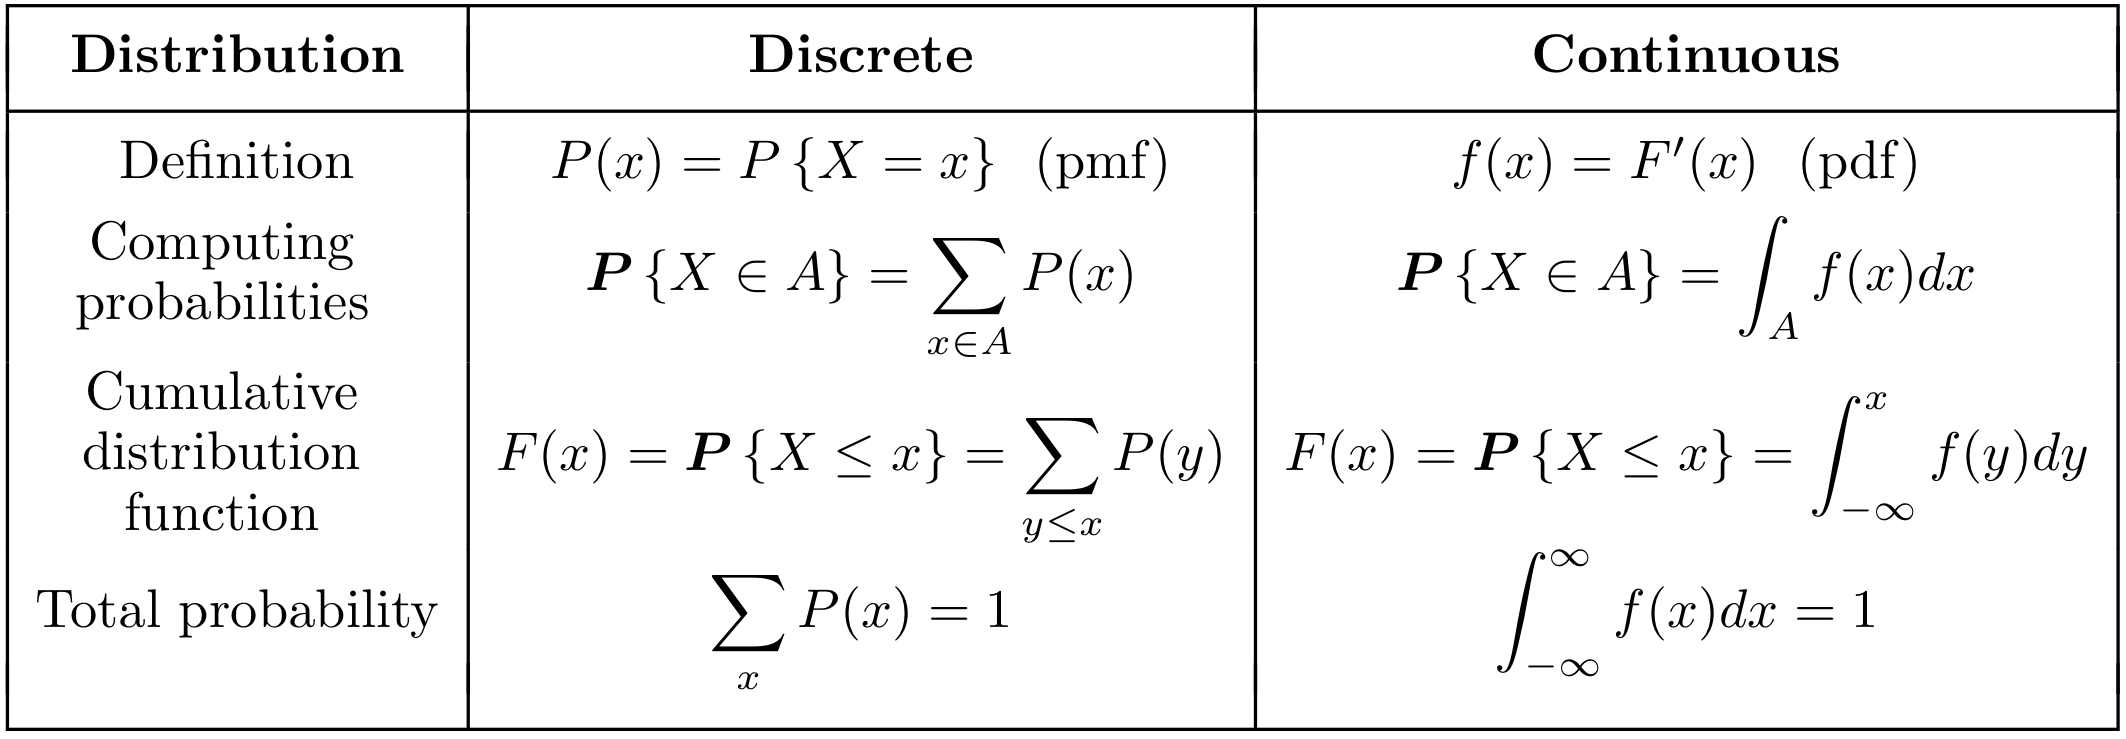
\includegraphics[width=1\linewidth]{images/pmf_cdf.jpeg}
\end{center}
\end{figure}

\begin{figure}[h]
\begin{center}
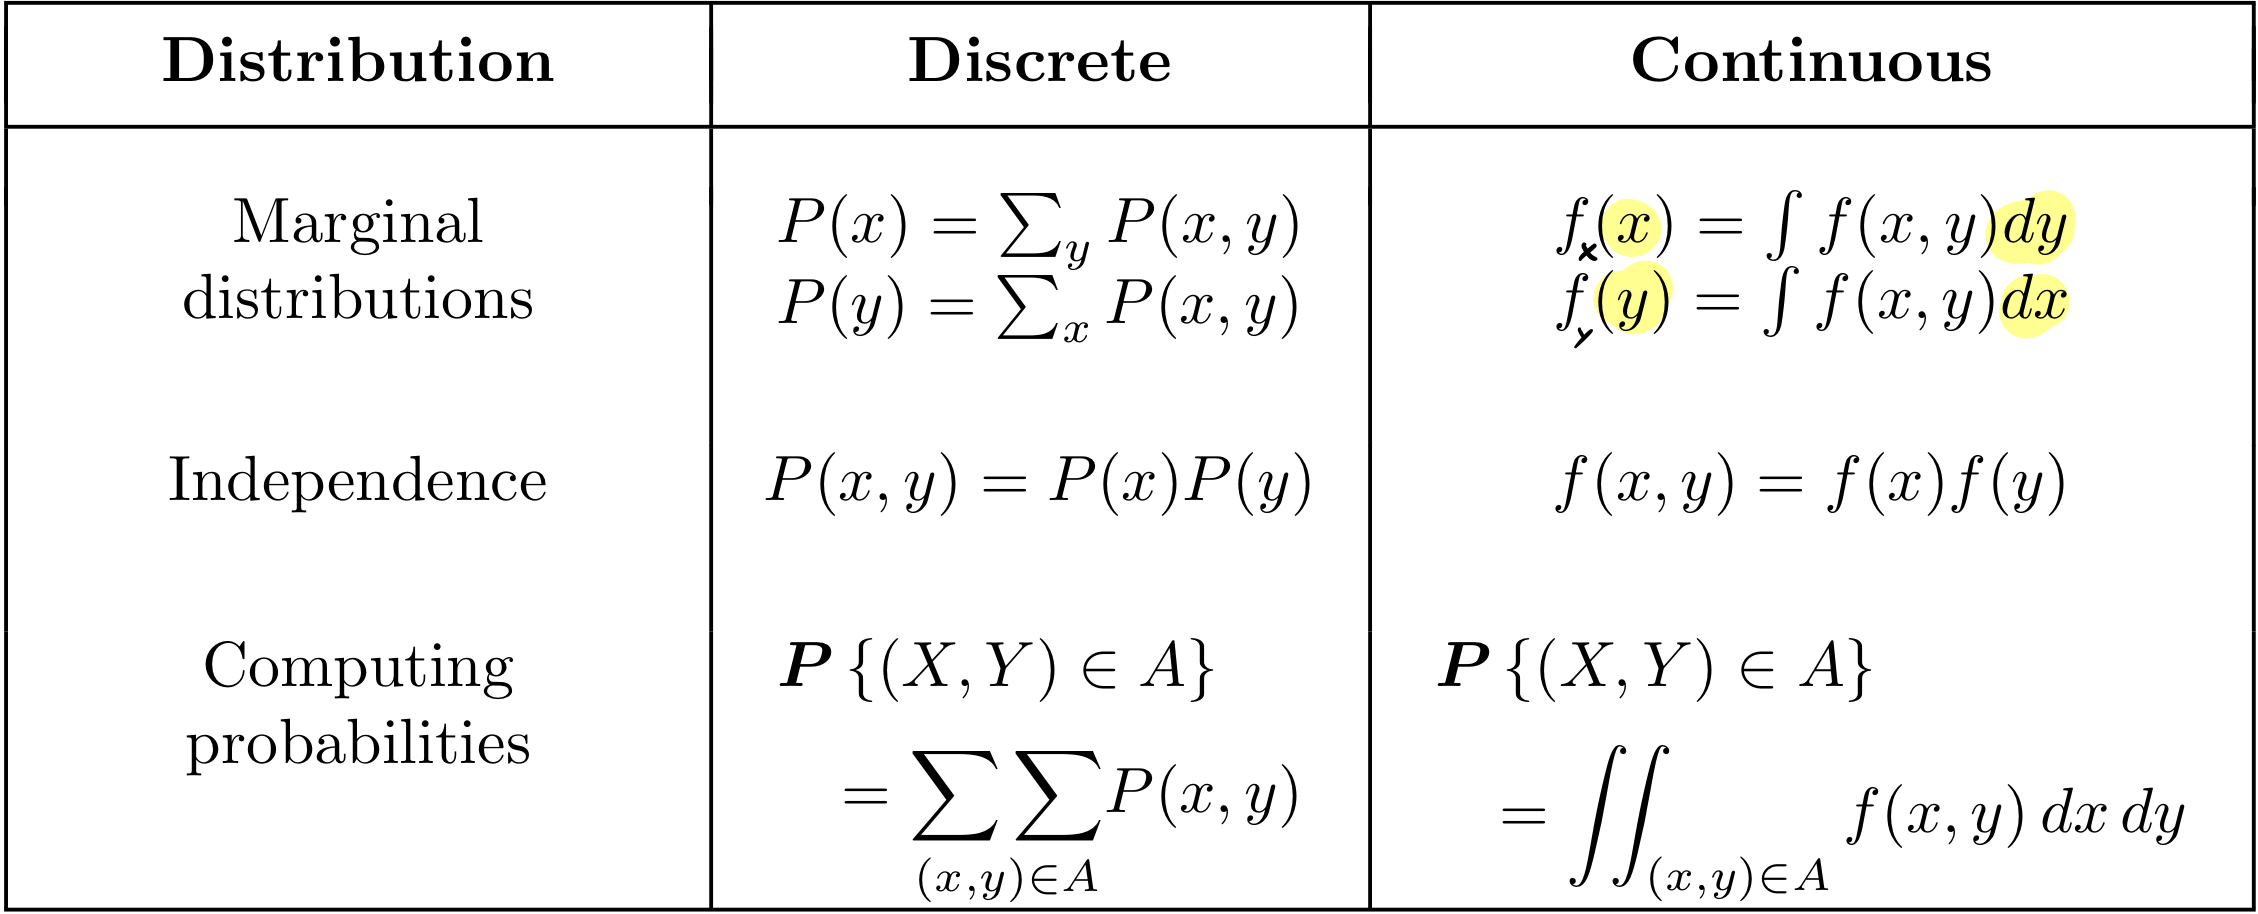
\includegraphics[width=1\linewidth]{images/marginal.jpeg}
\end{center}
\end{figure}

\textbf{Probabilità Condizionata}
\begin{itemize}
    \item \textit{Caso Discreto}
    $$P_{y|x}(y|x) = \frac{P_{xy}(x,y)}{P_{xx}(x)}$$
    $$P_{x|y}(x|y) = \frac{P_{xy}(x,y)}{P_{yy}(y)}$$
    Se $X$ e $Y$ sono indipendenti, allora
    $$P_{y|x}(y|x) = \frac{P_{xy}(x,y)}{P_{xx}(x)} = \frac{P_{xx}(x) \cdot P_{yy}(y)}{P_{xx}(x)} = P_{yy}(y)$$
    \item \textit{Caso Continuo}
    $$f_{y|x}(y|x) = \frac{f_{xy}(x,y)}{f_{xx}(x)}$$
    $$f_{x|y}(x|y) = \frac{f_{xy}(x,y)}{f_{yy}(y)}$$
    Se $X$ e $Y$ sono indipendenti, allora
    $$f_{y|x}(y|x) = \frac{f_{xy}(x,y)}{f_{xx}(x)} = \frac{f_{xx}(x) \cdot f_{yy}(y)}{f_{xx}(x)} = f_{yy}(y)$$
\end{itemize}

\begin{figure}[h]
\begin{center}
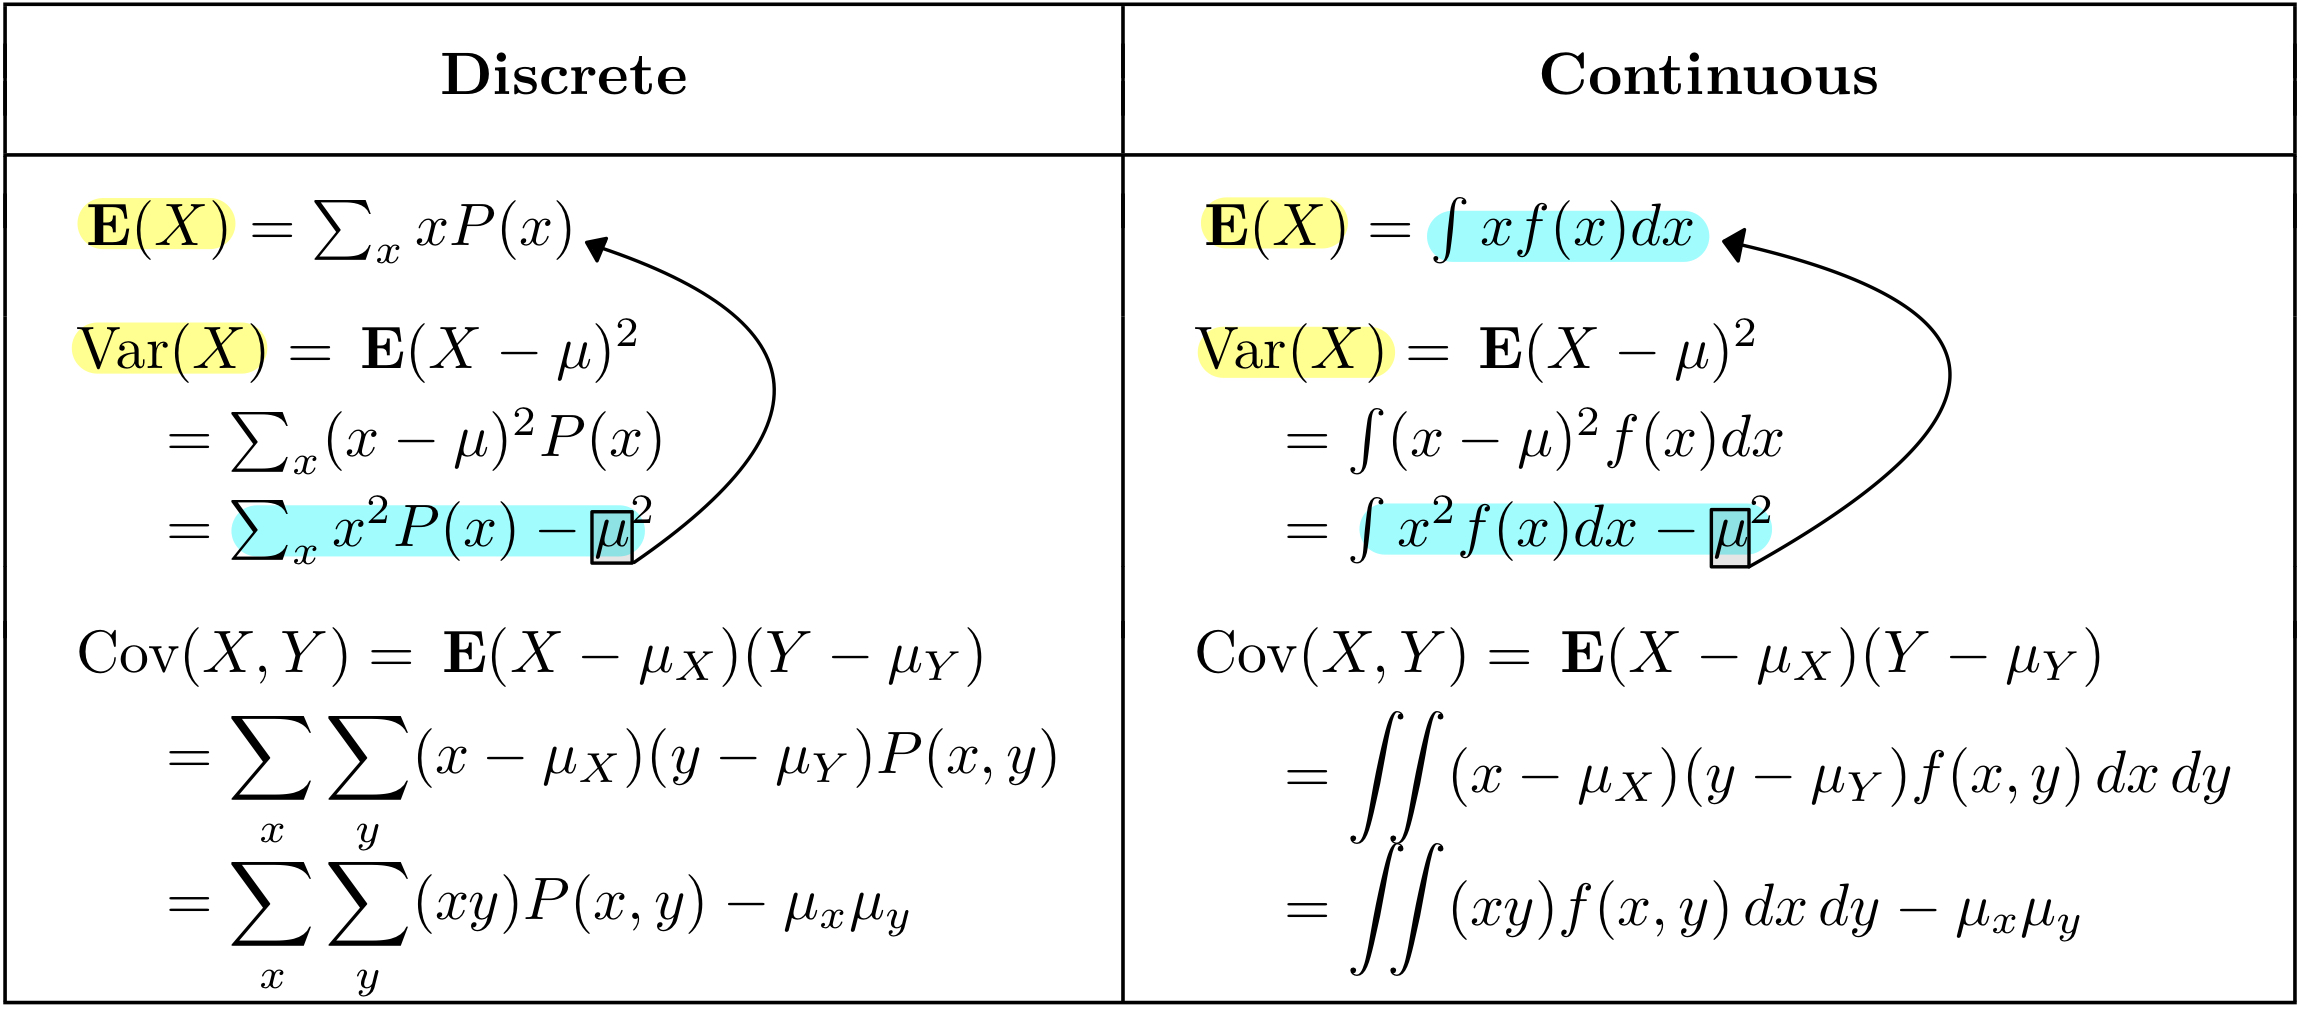
\includegraphics[width=1\linewidth]{images/e_var_cov.jpeg}
\end{center}
\end{figure}
%\chapter{Poisson Process}
\begin{tcolorbox}
\textbf{Poisson process} is a continuous-time counting stochastic process obtained from a Binomial counting process when its frame size $\Delta$ decreases to 0 while the arrival rate $\lambda$ remains constant. 
\end{tcolorbox}


\begin{itemize}
    \item \textbf{Marginal Distribution}
    $$N(t) \sim Po(\lambda t) \quad t > 0 \quad N(0) = 1$$

    \item \textbf{Transition Probabilities}
    $$
    \mathcal{P}_{m,n+m}(h) = \mathbb{P}[N(t+h) = n+m|N(t)=m] = \begin{cases} 1-\lambda h + o(h) & \mbox{if } n = 0 \\ 
    \lambda h + o(h) & \mbox{if } n = 1\\
    o(h) & \mbox{if } n > 1\\ \end{cases}
    $$

    \item \textbf{Transition Increments}
    \begin{align*}
    \mathcal{P}_{m,n+m}(h) &= \mathbb{P}[N(t+h) = n+m|N(t)=m] \\
    & = \mathbb{P}[N(t+h - t) = n+m - m|N(0)=0]\\
    & = \mathbb{P}[N(h) = n]\\
    & = \sum_{x=0}^n \frac{e^{-\lambda t} (\lambda t)^x}{x!} \text{ used also for }  \mathbb{P}[N(h) \leq n]
    \end{align*}

   \item \textbf{Independent Increments}
   $$(s_1, t_1) \cap (s_2, t_2) = \emptyset \rightarrow N(t_1) - N(s_1) \indep N(t_2) - N(s_2)$$
\end{itemize}

\begin{tcolorbox}
\textbf{Poisson Process}
    \begin{itemize}
        \item \(X(t) = Poisson(\lambda t) \text{ refer to propriety of the Pois with param. } \lambda t\) 
        \item \(T = Exponential(\lambda) \text{ refer to propriety of the Exp with param. } \lambda \)
        \item \(T_k = Gamma(k,\lambda) \text{ refer to propriety of the Gam with params. } \lambda \text{ and } k\)
        \item \(\mathbb{P}[T_k \leq t] = \mathbb{P}[X(t) \geq k]\)
        \item \(\mathbb{P}[T_k > t] = \mathbb{P}[X(t) < k]\)
    \end{itemize}
\end{tcolorbox}

\begin{figure}[h]
\begin{center}
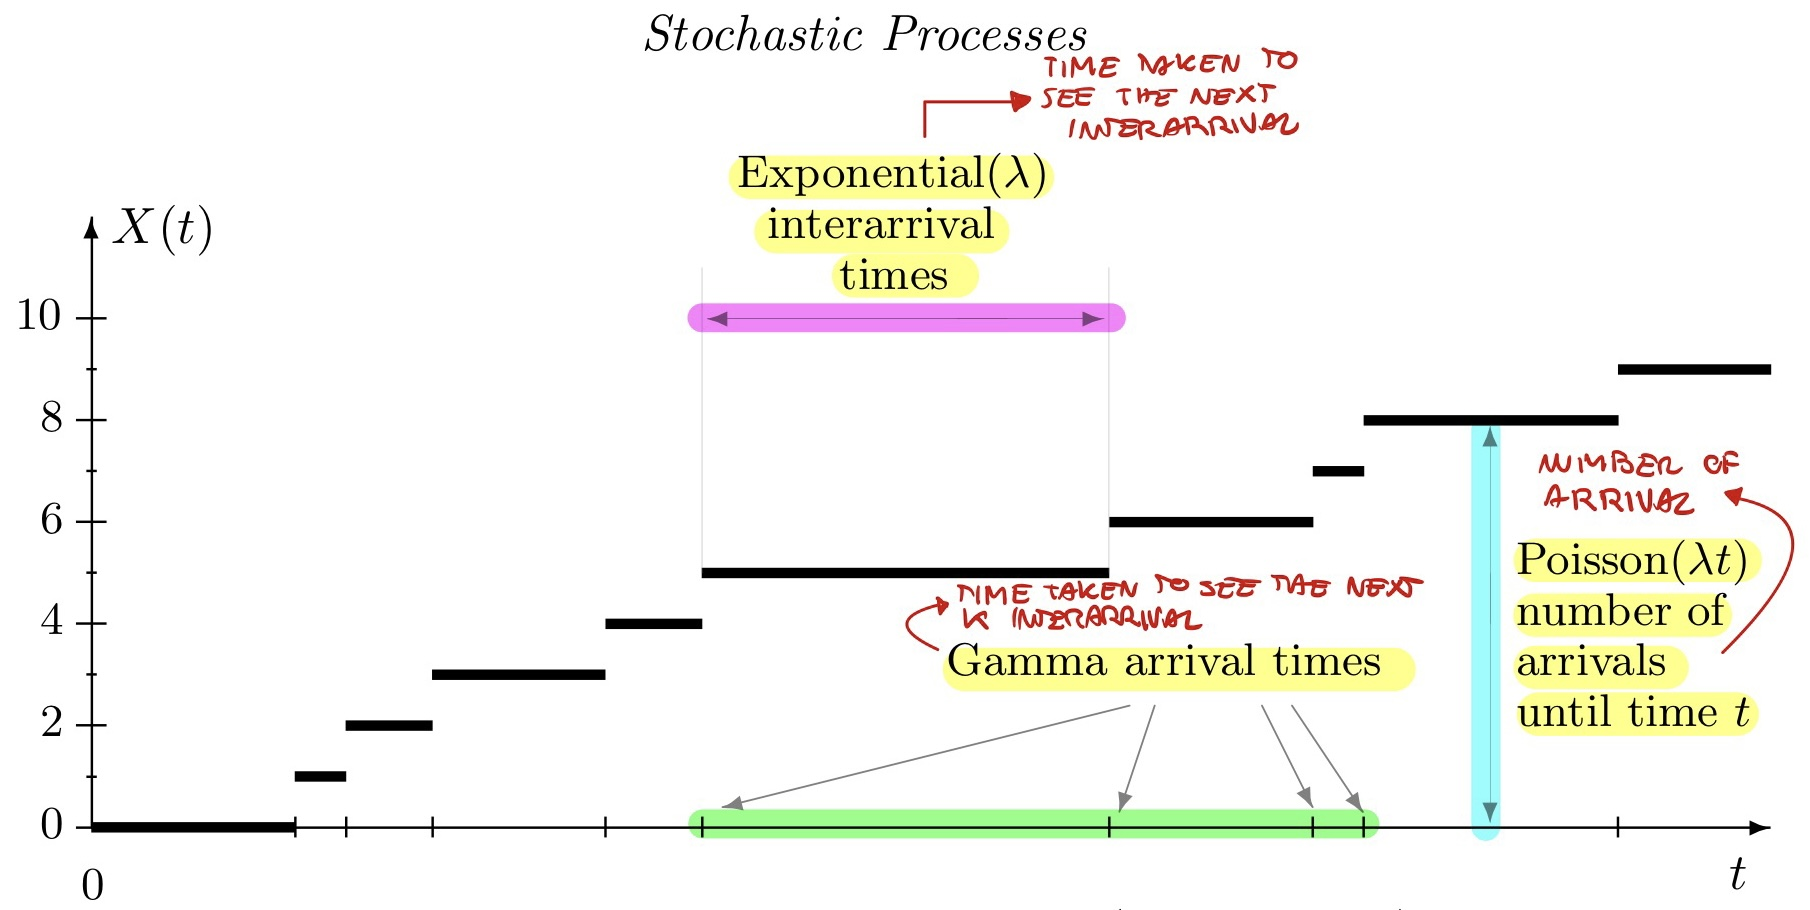
\includegraphics[width=1\linewidth]{images/poisson_process.jpeg}
\end{center}
\end{figure}

\section{Definitions}
\subsection{Definition 1}
A Poisson Process with intensity $\lambda$ is a \textit{Continuous-Time Counting Process} $N=\{N(t): t \geq 0\}$ taking values in $S = \{0,1,2,...\} = \mathbb{N}$ s.t.:
\begin{enumerate}
    \item $N(0) = 0$
    \item \textbf{The increments are independent and stationary} st $N(t+h) - N(t)$ depends only on $h$
    \item $P[N(h) = 1] = \lambda h + o(h)$ and $P[N \geq 2] = o(h)$
\end{enumerate}

\subsection{Definition 2}
A Poisson Process with intensity $\lambda$ is a \textit{Continuous-Time Counting Process} $N=\{N(t): t \geq 0\}$ s.t.
\begin{enumerate}
    \item $N(0) = 0$
    \item For each non overlapping time intervals $(s_1, s_1+t_1]$ and $(s_2, s_2+t_2]$ for $t_1,t_2,s_1,s_2 \geq 0$ the increments $N(s_1+t_1) - N(s_1)$ and $N(s_2+t_2) - N(s_2)$ are \textbf{independent}
    \item $\forall t,s \geq 0$ the \textbf{increment} $N(t+s) - N(s)$ has a \textbf{Poisson} $(\lambda t)$ distribution
\end{enumerate}

\subsection{Definition 3}
A Poisson Process with intensity $\lambda$ is a \textit{Continuous-Time Counting Process} $N=\{N(t): t \geq 0\}$ s.t.
\begin{enumerate}
    \item $N(0) = 0$
    \item Let $T_0 = 0$ and $\forall n \geq 1$ $T_n = inf\{t:N(t) = n\}$ be the n-th arrival time, then the \textbf{nterarrival times} $X_n = T_n - T_{n-1}$ are \textit{iid} \textbf{exponential random variables} with rate $\lambda$
\end{enumerate}

\section{Proprieties}
\subsection{Superposition}
$$N_i \stackrel{\text{iid}}{\sim} PP(\lambda_i) \rightarrow N = \sum_{i=1}^\infty N_i \sim PP(\lambda) \quad \text{where} \quad \lambda = \sum_{i=1}^\infty \lambda_i \text{ must be finite}$$

\subsection{Thinning}
$N \sim PP(\lambda)$ and each arrival assigned to process $N_i$ with probability $p_i$ independently from all others for $p_i \in (0,1)$ such that:
$$\sum_{i=1}^\infty p_i = 1 \quad \quad N_i \stackrel{\text{ind}}{\sim} PP(\lambda \cdot p_i)$$

\subsection{Auto-covariance - $\sigma(s,t) = COV(N(s), N(t))$}
\begin{itemize}
    \item If $s > t$ we split into $[0,s) = [0,t) \cup (t,s]$
    \begin{align*}
    COV(N(t), N(s)) = & COV(N(t), N(t) + N(s) - N(t)))\\
    & COV(N(t),N(t)) + COV(N(t), N(s) - N(t))\\
    & VAR(N(t)) + 0 = \lambda t
    \end{align*}
    \item If $t > s$ we split into $[0,t) = [0,s) \cup (s,t]$
    \begin{align*}
    COV(N(s), N(t)) = & COV(N(s) + N(t) - N(s), N(t)))\\
    & COV(N(s),N(s)) + COV(N(t) - N(s), N(s))\\
    & VAR(N(s)) + 0 = \lambda s
    \end{align*}
\end{itemize}
Thus we obtain that the auto-covariance is equal to 
$$\sigma(s,t) = COV(N(s), N(t)) = \lambda(min\{s,t\})$$


%\chapter{Random Variables}

\begin{figure}[h]
\begin{center}
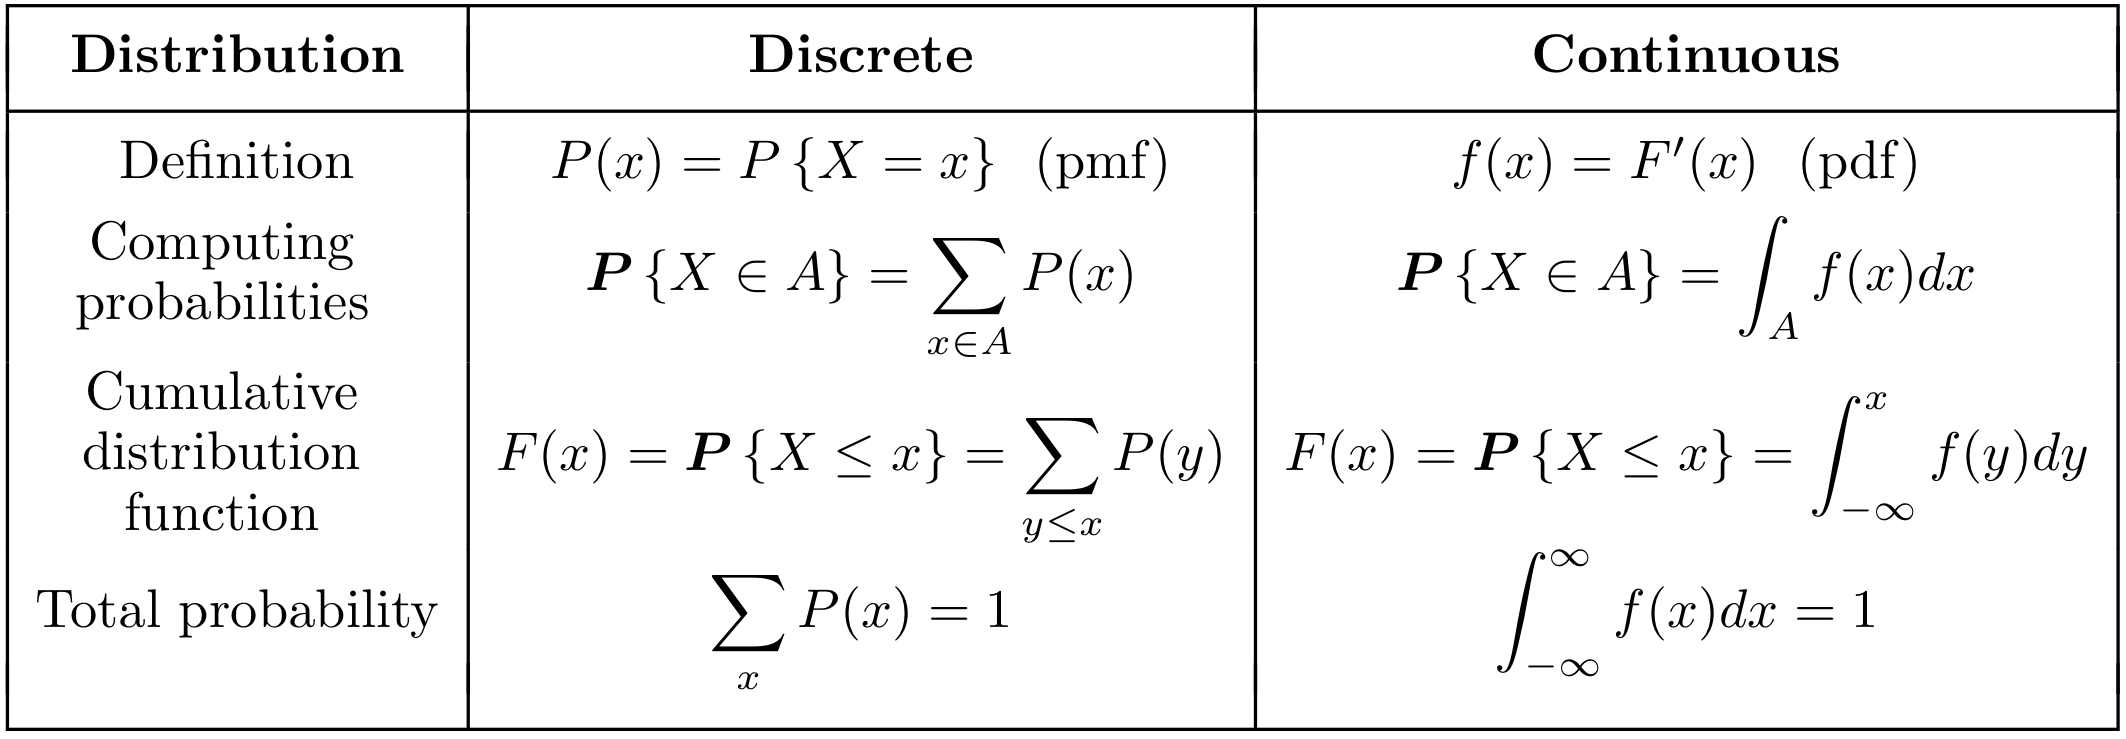
\includegraphics[width=1\linewidth]{images/pmf_cdf.jpeg}
\end{center}
\end{figure}

\begin{figure}[h]
\begin{center}
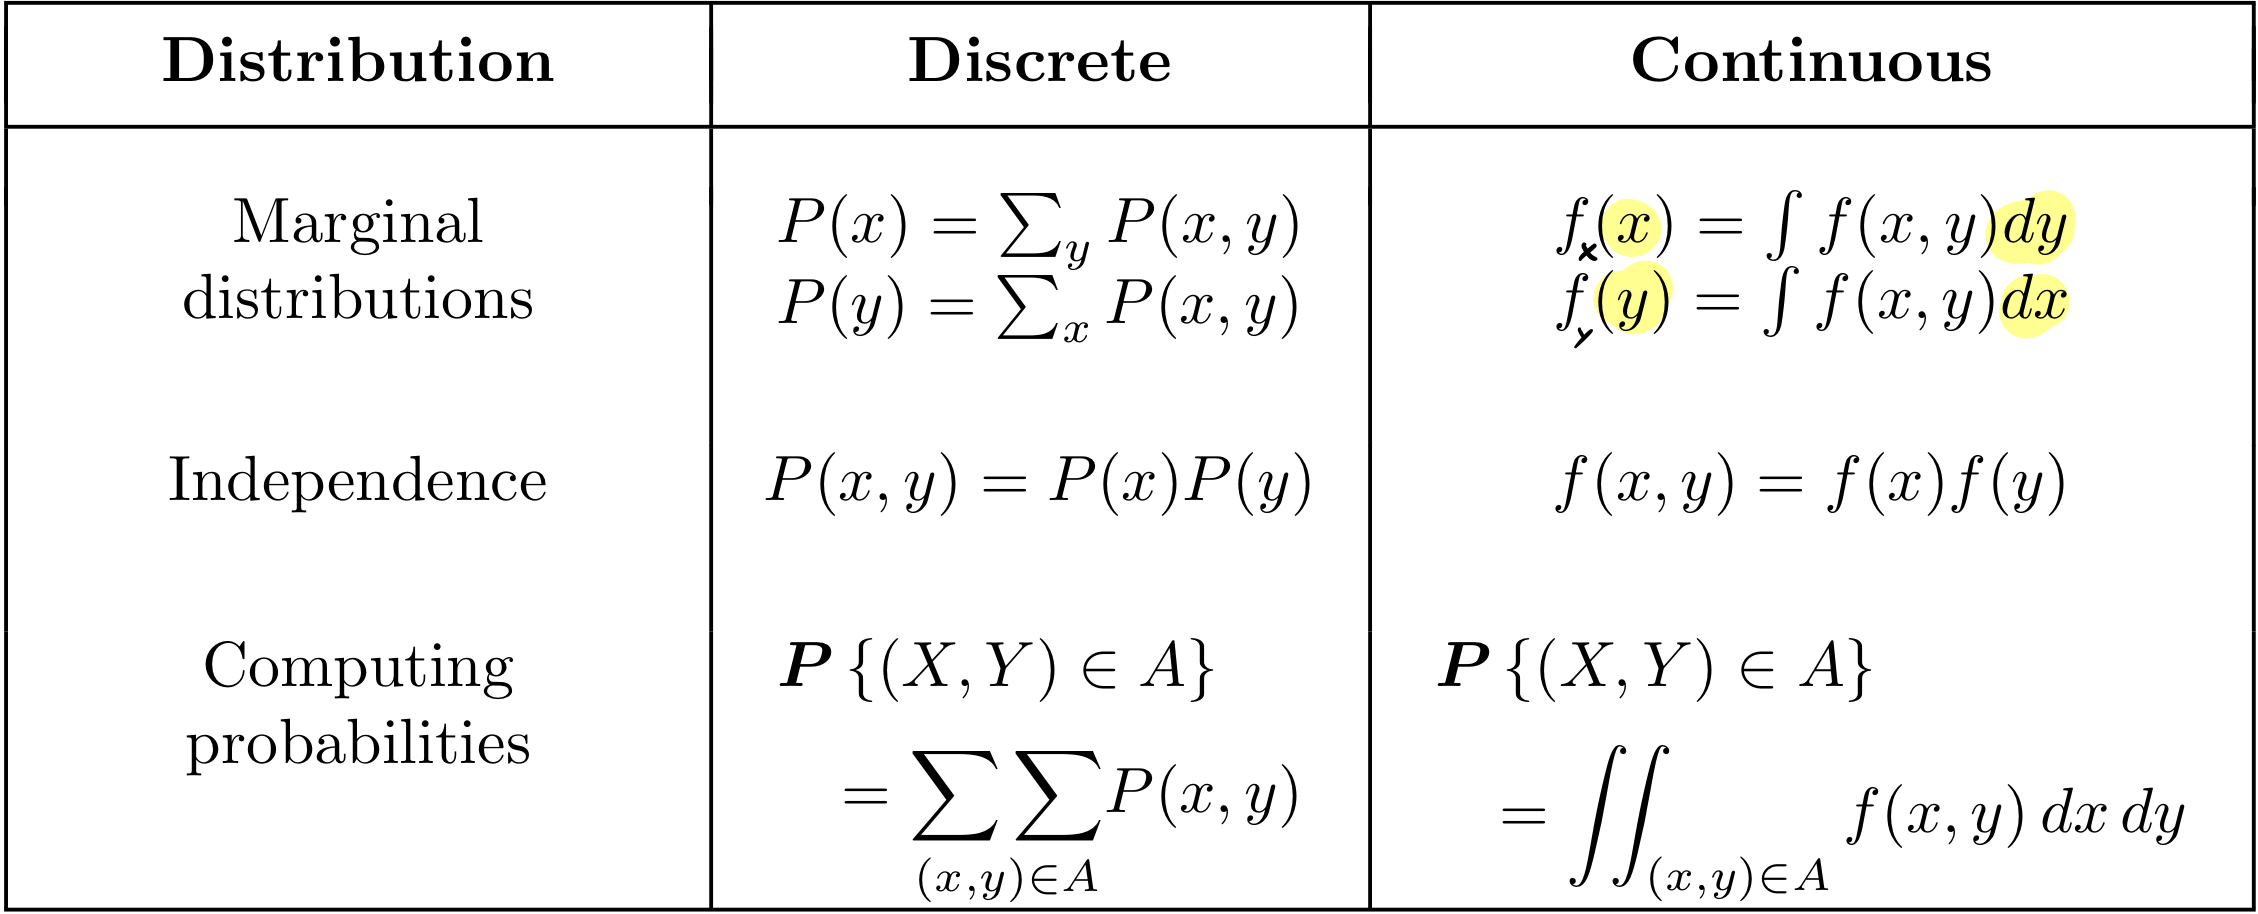
\includegraphics[width=1\linewidth]{images/marginal.jpeg}
\end{center}
\end{figure}

\textbf{Conditional Probability}
\begin{itemize}
    \item \textit{Discrete case}
    $$P_{y|x}(y|x) = \frac{P_{xy}(x,y)}{P_{xx}(x)}$$
    $$P_{x|y}(x|y) = \frac{P_{xy}(x,y)}{P_{yy}(y)}$$
    If $X$ and $Y$ are independent, then
    $$P_{y|x}(y|x) = \frac{P_{xy}(x,y)}{P_{xx}(x)} = \frac{P_{xx}(x) \cdot P_{yy}(y)}{P_{xx}(x)} = P_{yy}(y)$$
    \item \textit{Continuous case}
    $$f_{y|x}(y|x) = \frac{f_{xy}(x,y)}{f_{xx}(x)}$$
    $$f_{x|y}(x|y) = \frac{f_{xy}(x,y)}{f_{yy}(y)}$$
    If $X$ and $Y$ are independent, then
    $$f_{y|x}(y|x) = \frac{f_{xy}(x,y)}{f_{xx}(x)} = \frac{f_{xx}(x) \cdot f_{yy}(y)}{f_{xx}(x)} = f_{yy}(y)$$
\end{itemize}

\begin{figure}[h]
\begin{center}
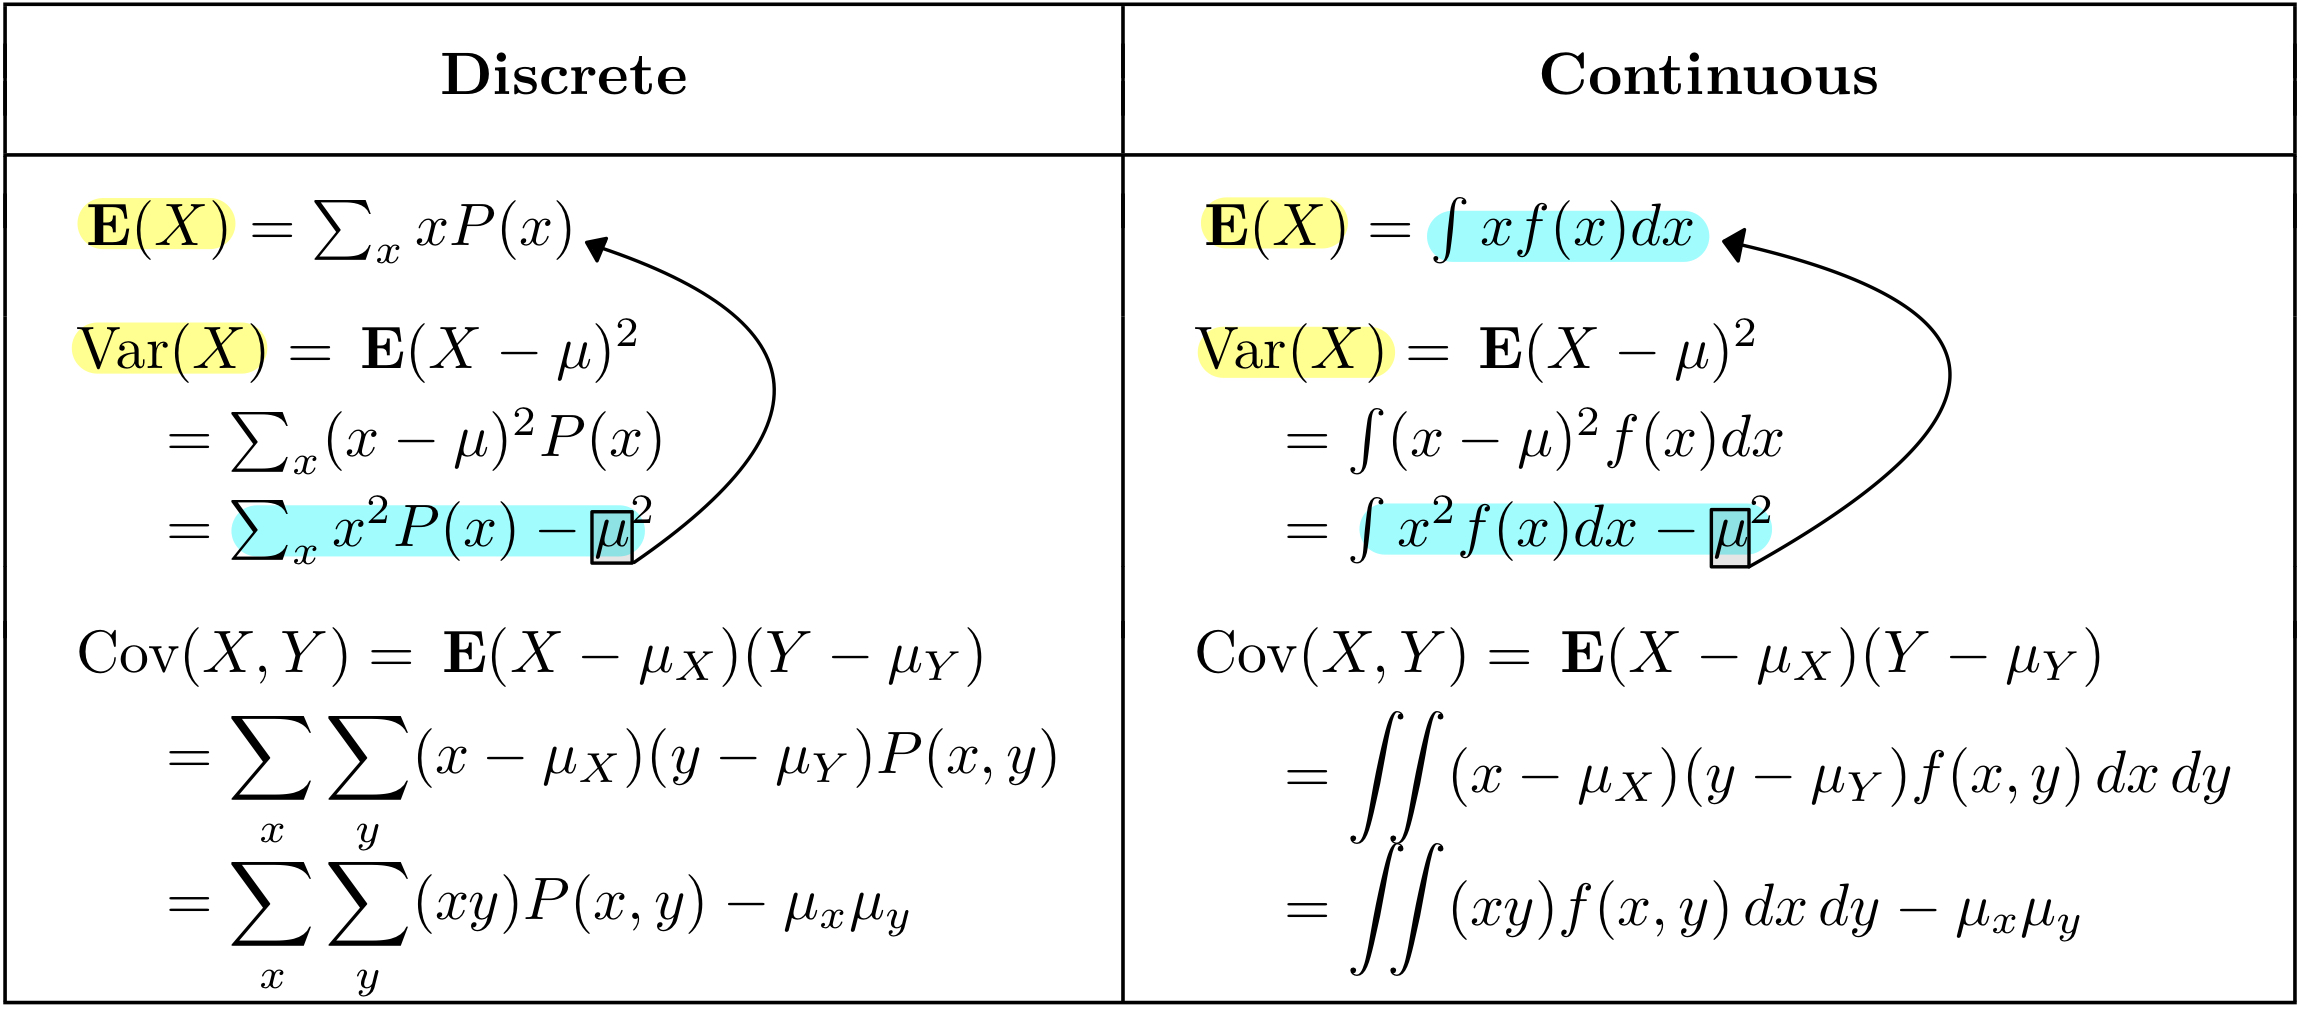
\includegraphics[width=1\linewidth]{images/e_var_cov.jpeg}
\end{center}
\end{figure}
%\chapter{Function Properties}
\section{Mean}
\begin{itemize}
    \item \(\mathbb{E}[aX +bY + c] = a\mathbb{E} + b\mathbb{E} + c\)
    \item \(\mathbb{E}[X + Y] = \mathbb{E}[X] + \mathbb{E}[Y]\)
    \item \(\mathbb{E}[X] = a\mathbb{E}[X]\)
    \item \textbf{For independent \(X\) and \(Y\)} \(\mathbb{E}[XY] = \mathbb{E}[X] \times \mathbb{E}[Y]\)
    \item \(X_1,X_2,...,X_n\) RVs, then \(\mathbb{E}[X_1 + X_2 + ... + X_n] = \mathbb{E}[X_1] + \mathbb{E}[X_2] + ... + \mathbb{E}[X_n] = \sum_{i=1}^n X_i\)
\end{itemize}

\section{Variance}
\begin{itemize}
    \item \(\mathbb{VAR}[X] = \mathbb{E}[X^2] - \mathbb{E}[X]^2\)
    \item \(\mathbb{VAR}[X + c] = \mathbb{VAR}[X] \quad \quad \mathbb{VAR}[cX] = c^2\mathbb{VAR}[X]s\)
    \item \(\mathbb{VAR}[aX + bY + c] = a^2\mathbb{VAR}[X] + b^2\mathbb{VAR}[Y] + 2ab\mathbb{COV}[X, Y]\)
    \item \textbf{For independent \(X\) and \(Y\)} \(\mathbb{VAR}[X + Y] = \mathbb{VAR}[X] + \mathbb{VAR}[Y]\)
\end{itemize}

\section{Covariance}
\begin{itemize}
    \item \(\mathbb{VAR}[X] = COV[X,X]\)
    \item \(\mathbb{COV}[cX,Y] = c\mathbb{COV}[X,Y] \quad 
 \quad \mathbb{COV}[X,cY] = c\mathbb{COV}[X,Y]\)
    \item \(\mathbb{COV}[X + Y, Z] = \mathbb{COV}[X,Z] + \mathbb{COV}[Y,Z]\)
    \item \(\mathbb{COV}[X, Y + Z] = \mathbb{COV}[X,Y] + \mathbb{COV}[X,Z]\)
    \item \(\mathbb{COV}[X,Y] = \mathbb{COV}[Y,X]\)
    \item \(\mathbb{COV}[X,c] = 0\)
    \item \textbf{For independent \(X\) and \(Y\)} \(\mathbb{COV}[X,Y] = 0\)
    \item \(\mathbb{COV}[X + Y, Z + W] = \mathbb{COV}[X,Y] + \mathbb{COV}[X,W] + \mathbb{COV}[Y,Z] + \mathbb{COV}[Y,W]\)
\end{itemize}
%\chapter{VA Discrete}

\section{Distribuzione di Bernoulli}
\begin{tcolorbox}
Utilizzato ogni volta che abbiamo un risultato 0/1, quindi quando potremmo avere solo due possibili risultati nel nostro esperimento.
\end{tcolorbox}

\begingroup
\setlength{\tabcolsep}{10pt} % Default value: 6pt
\renewcommand{\arraystretch}{1.5} % Default value: 1
\begin{center}
\begin{tabular}{ |c|c| } 
\hline
\(p\) & probabilità di successo \\ \hline
\(P[X]\) & $p^x(1 - p)^{1-x} = \begin{cases} 1 - p & \mbox{if } x = 0 \\p & \mbox{if } x = 1 
\end{cases}$ \\ \hline
\(\mathbf{E}[X]\) & $p$ \\ \hline
\(\text{VAR}[X]\) & $p(1 - p)$ \\ \hline
\end{tabular}
\end{center}
\endgroup





\section{Distribuzione Binomiale}
\begin{tcolorbox}
Utilizzato ogni volta che consideriamo una sequenza di prove Bernoulliane indipendenti e contiamo il numero di successi in essa contenuti.
\end{tcolorbox}
\begingroup
\setlength{\tabcolsep}{10pt} % Default value: 6pt
\renewcommand{\arraystretch}{1.5} % Default value: 1
\begin{center}
\begin{tabular}{ |c|c| } 
\hline
\(n\) & numero di osservazioni \\ \hline
\(p\) & probabilità di successo \\ \hline
\(P[x]\) & $\dbinom{n}{x} p^x(1-p)^{n - x}$\\ \hline
\(F[x]\) & $\sum_{i = 1}^n \dbinom{n}{i} p^i(1 - p)^{n-i}$ \\ \hline
\(\mathbf{E}[X]\) & \(np\) \\ \hline
VAR\([X]\) & \(np(1 - p)\) \\ \hline\hline
\(P[X = x]\) & \begin{lstlisting}[language=R]
dbinom(#success, size, prob_success)
\end{lstlisting} \\ \hline
\(P[X \leq x]\) & \begin{lstlisting}[language=R]
pbinom(#success, size, prob_success)
\end{lstlisting} \\ \hline
\end{tabular}
\end{center}
\endgroup




\section{Distribuzione Geometrica}
\begin{tcolorbox}
Considera una sequenza di prove Bernoulliane indipendenti, ciascuna prova si traduce in un "successo" o un "fallimento". Il numero di prove Bernoulliane necessarie per ottenere il primo successo ha distribuzione geometrica.
\end{tcolorbox}
\begingroup
\setlength{\tabcolsep}{10pt} % Default value: 6pt
\renewcommand{\arraystretch}{1.5} % Default value: 1
\begin{center}
\begin{tabular}{ |c|c| } 
\hline
\(p\) & probabilità di successo \\ \hline
\(P[x]\) & \((1 - p)^{x-1}p, x = 1,2,...\)\\ \hline
\(F[x]\) & \(p \sum_{i = 0}^x (1 - p)^i\) \\ \hline
\(\mathbf{E}[X]\) & \(\frac{1}{p}\) \\ \hline
VAR\([X]\) & \(\frac{1-p}{p^2}\) \\ \hline\hline
\(P[X = x]\) & \begin{lstlisting}[language=R]
dgeom(#failures, prob_success)
\end{lstlisting} \\ \hline
\(P[X \leq x]\) & \begin{lstlisting}[language=R]
pgeom(#failures, prob_success)
\end{lstlisting} \\ \hline
\end{tabular}
\end{center}
\endgroup

\subsection{Memory Less Propriety}
Se \(X \sim Geo(p)\) allora
\[\mathbb{P}[X > m + n | X > m] \frac{\mathbb{P}[X > m + n]}{\mathbb{P}[X > n]}\]
Questa proprietà si dimostra tenendo conto che
\[\mathbb{P}[X > k] = (1 - p)^k \quad k = 0,1,2,...\]


\newpage
\section{Distribuzione IperGeometrica}
\begin{tcolorbox}
Descrive la probabilità di \(k\) successi (estrazioni casuali per le quali l'oggetto disegnato ha una caratteristica specificata) in \(n\) estrazioni, senza reinserimento, da una popolazione finita di dimensione \(N\) che contiene esattamente \( K\) oggetti con quella caratteristica, in cui ogni pareggio è un successo o un fallimento.
\end{tcolorbox}
\begingroup
\setlength{\tabcolsep}{10pt} % Default value: 6pt
\renewcommand{\arraystretch}{1.5} % Default value: 1
\begin{center}
\begin{tabular}{ |c|c| } 
\hline
\(N\) & Dimensione della popolazione \\ \hline
\(K\) & Numero di successi nella popolazione \\ \hline
\(n\) & Numero di campionamenti  \\ \hline
\(k\) & Numero di successi osservati \\ \hline
\(P[x]\) & \(\frac{\dbinom{K}{k}\dbinom{N-K}{n-k}}{\dbinom{N}{n}}\)\\ \hline
\(\mathbf{E}[X]\) & \(n \cdot \frac{K}{N}\) \\ \hline
VAR\([X]\) & \(n \cdot \frac{K}{N} \cdot\frac{N-K}{N} \cdot \frac{N-n}{N-1}\) \\\hline\hline
\(P[X = x]\) & \begin{lstlisting}[language=R]
dhyper(#succ, #succ_samp, #pop_dim, #samp_dim)
\end{lstlisting} \\ \hline
\(P[X \leq x]\) & \begin{lstlisting}[language=R]
phyper(#succ, #succ_samp, #pop_dim, #samp_dim)
\end{lstlisting} \\ \hline
\end{tabular}
\end{center}
\endgroup



\section{Distribuzione Multinomiale}
\begin{tcolorbox}[title=NOTA]
Il seguente paragrafo è opzionale, non è richiesto per l'esame!
\end{tcolorbox}
\begin{tcolorbox}
Mentre la distribuzione binomiale descrive il numero di successi in un processo di Bernoulli, per il quale ogni singolo test può fornire solo due risultati, la distribuzione multinomiale descrive il caso più generale in cui ogni test può fornire un numero finito di risultati, ciascuno con la propria probabilità.
\end{tcolorbox}
\[P[X_1, X_2,...,X_k] = \frac{n!}{x_1!...x_k!}p_1^{x_1}...p_k^{x_k} \quad \text{dove} \quad \sum_{i = 1}^n p_1 = 1\]


\newpage
\section{Distribuzione Binomiale Negativa}
\begin{tcolorbox}[title=NOTA]
Il seguente paragrafo è opzionale, non è richiesto per l'esame!
\end{tcolorbox}
\begin{tcolorbox}
In una sequenza di prove Bernoulliane indipendenti, il numero di prove necessarie per ottenere \(k\) successi ha distribuzione binomiale negativa.

In altre parole conta il numero di fallimenti prima di ottenere un numero target di successi (k).
\end{tcolorbox}
\begingroup
\setlength{\tabcolsep}{10pt} % Default value: 6pt
\renewcommand{\arraystretch}{1.5} % Default value: 1
\begin{center}
\begin{tabular}{ |c|c| } 
\hline
\(k\) & Numero di successi \\ \hline
\(p\) & Probabilità di successo \\ \hline
\(P[x]\) & $\dbinom{x - 1}{k - 1}(1 - p)^{x - k}p^k \quad x = k, k+1,...$\\ \hline
\(\mathbf{E}[X]\) & \(\frac{k}{p}\) \\ \hline
VAR\([X]\) & \(\frac{k(1 - p)}{p^2}\) \\ \hline\hline
\(P[X = x]\) & \begin{lstlisting}[language=R]
dnbinom(#failures, #successes, prob_success)
dnbinom(#trial-#successes, #successes, prob_success)
\end{lstlisting} \\ \hline
\(P[X \leq x]\) & \begin{lstlisting}[language=R]
pnbinom(#failures, #successes, prob_success)
pnbinom(#trial-#successes, #successes, prob_success)
\end{lstlisting} \\ \hline
\end{tabular}
\end{center}
\endgroup

\newpage
\section{Distribuzione di Poisson}
\begin{tcolorbox}
    Poisson è legata agli \textbf{eventi rari}. Ciò significa che è estremamente improbabile che due eventi si verifichino contemporaneamente o in un periodo di tempo molto breve.

    Il numero di eventi rari che si verificano in un determinato periodo di tempo ha una distribuzione di Poisson.
\end{tcolorbox}

\begingroup
\setlength{\tabcolsep}{10pt} % Default value: 6pt
\renewcommand{\arraystretch}{1.5} % Default value: 1
\begin{center}
\begin{tabular}{ |c|c| } 
\hline
\(\lambda\) & Frequenza, numero medio di eventi \\ \hline
\(p\) & Probabilità di successo \\ \hline
\(P[x]\) & $e^{-\lambda} \frac{\lambda^x}{x!} \quad x = 0,1,2,...$\\ \hline
\(\mathbf{E}[X]\) & \(\lambda\) \\ \hline
VAR\([X]\) & \(\lambda\) \\ \hline\hline
\(P[X = x]\) & \begin{lstlisting}[language=R]
dpois(x, lambda)
\end{lstlisting} \\ \hline
\(P[X \leq x]\) & \begin{lstlisting}[language=R]
ppois(x, lambda)
\end{lstlisting} \\ \hline
\end{tabular}
\end{center}
\endgroup


\subsection{Approssimazione della Binomiale tramite Poisson}
La distribuzione di Poisson può essere utilizzata efficacemente per approssimare le probabilità binomiali quando il \textit{numero di prove} \(n\) è \textbf{grande} e la \textit{probabilità di successo} \(p\) è \textbf{piccola}
\[n \geq 30 \quad p \leq 0.05\]

\[\text{Binomiale}(n,p) \approx \text{Poisson}(\lambda)\]
\[\text{dove } n \geq 30 \quad p \leq 0.05 \quad np=\lambda\]

\subsection{Proprietà Additiva}
Se
\[X \sim Pois(\lambda) \quad \text{and} \quad Y \sim Pois(\mu)\]
e sono \textbf{indipendenti}, dopo possiamo dire che:
\[W = X + Y \sim Pois(\lambda + \mu)\]

\subsection{Relazione tra Poisson e Distribuzione Multinomiale}
\begin{tcolorbox}[title=NOTA]
Il seguente paragrafo è opzionale, non è richiesto per l'esame!
\end{tcolorbox}
Sia 
\[S_n = X_1 + X_2 + ... + X_n \quad \text{with} \quad X_i\stackrel{iid}{\sim} Pois(\lambda_i)\]
dato
\[(X_1,X_2,...,X_n)|S_n \sim Mult\Big(\frac{\lambda_1}{\lambda},\frac{\lambda_2}{\lambda},...,\frac{\lambda_n}{\lambda}\Big) \quad \text{dove} \quad \lambda = \sum_{i = 1}^n \lambda_i\]
%\chapter{Approximation}
Given \(X_1,X_2,...,X_n\) a sequence of independent random variables with \(S_n = \sum_{i = 1}^n X_i\) if:
\begin{itemize}
    \item \(X_i \stackrel{iid}{\sim} \text{Bernulli}(p) \approx S_n \sim \text{Binomial}(n,p)\)
    \item \(X_i \stackrel{iid}{\sim} \text{Geometric}(p) \approx S_n \sim \text{NegativeBinomial}(n,p)\)
    \item \(X_i \stackrel{iid}{\sim} \text{Exponential}(\lambda) \approx S_n \sim \text{Gamma}(\alpha=n,\lambda)\)
    \item \(X_i \stackrel{iid}{\sim} \text{Poisson}(\lambda) \approx S_n \sim \text{Poisson}(n*\lambda)\)
\end{itemize}
%\chapter{Stochastic Processes}
\begin{tcolorbox}
A \textbf{Stochastic Process} is a Random Variable that also depends on \textbf{time}, thus it is a function of two arguments \(X(t,w)\) where:
\begin{itemize}
    \item \(t \in \mathcal{T}\) is \textbf{time}
    \item \(w \in \Omega\)
\end{itemize}
Moreover:
\begin{itemize}
    \item At any time \(t\) we see a \textbf{random variable} \(X_t(w)\): function of random income.
    \item At a given \(w\) we obtain a \textbf{function of time} \(X_w(t)\)
\end{itemize}
\end{tcolorbox}

We have two classification of stochastic processes and are the following one:
\begin{itemize}
    \item \textbf{Variable Classification:}
    \begin{itemize}
        \item \(X(t,w)\) is a \textbf{discrete-state process} if \(X_t\) is a \textit{discrete rv} \(\forall t\)
        \item \(X(t,w)\) is a \textbf{continuous-state process} if \(X_t\) is a \textit{continuous rv} \(\forall t\)
    \end{itemize}
    \item \textbf{Time Dimension Classification:}
    \begin{itemize}
        \item \(X(t,w)\) is a \textbf{discrete-state process} if the set of time \(\mathcal{T}\) is \textit{discrete}
        \item \(X(t,w)\) is a \textbf{continuous-state process} if \(\mathcal{T}\) is unbounded and thus \textit{continuous} 
    \end{itemize}
\end{itemize}

\section{Proprieties}
\subsection{Mean Function}
\[\mu_x(t) = \mathbb{E}[X(t)]\]
Where \(\mathbb{E}[X(t)]\) si the \textbf{expected value} of the rv for the fixed \textit{time point} \(t\)

\subsection{Variance Function}
\[\sigma^2(t) = VAR[X(t)] = \mathbb{E}[(X(t) - \mu_x(t))^2] = \mathbb{E}[X^2(t)] - [\mu_x(t)]^2\]

\subsection{Standard Deviation Function}
\[\sigma_x(t) = \sqrt{VAR[X(t)]} = \sqrt{\sigma_x^2(t)}\]

\subsection{Auto-Covariance Function}
\[\sigma_x(t,s) = C_{x,x} = COV[X(t), X(s)] = \mathbb{E}\Big[\Big(X(t) - \mu_x(t)\Big) \times \Big(X(s) - \mu_x(s)\Big)\Big]\]
\[ = \mathbb{E}\Big[\Big(X(t) \times X(s)\Big) - \Big(\mu_x(t) \times \mu_x(s)\Big)\Big]\]

And it has the following proprieties:
\begin{itemize}
    \item \(C_{x,x}(t,s) = C_{x,x}(s,t)\)
    \item \(\sigma^2_x(t) = VAR[X(t)] = COV[X(t),X(t)] = C_{x,x}(t,t) = \mathbb{E}[X^2(t)] - u^2_x(t)\)
    \item It is interpreted as the classic covariance
\end{itemize}

\subsection{Auto-Correlation Function}
\[\varphi_x(t,s) = \frac{\sigma_x(t,s)}{\sigma_x(t)\sigma_x(s)} = \frac{C_{x,x}(t,s)}{C_{x,x}(t)C_{x,x}(s)} = \frac{\text{autocovariance}}{\text{SD of s times SD of t}}\]
In context of \textbf{signal processing} ad in \textbf{engineering literature} the \textbf{autocorrelation functon} is denoted as \(R_{x,x}(t,s)\) and is defined as:
\[R_{x,x}(t,s) = \mathbb{E}[X(t)X(s)]\]
And it is equivalent to \(\sigma_x(t,s)\) only when the mean = 0 and the variance = 1

\section{Stationary and wide-sense stationary processes}
\subsection{Strongly / Strict-Sense Stationary}
\begin{tcolorbox}
A stochastic process is called \textbf{Strongly / Strict-Sense Stationary} if:
\begin{itemize}
    \item All its \textit{statistical proprieties} are \textbf{invariant over time}
    \item for any points \(t_1,...,t_r\) and any value \(\tau\) if the two following \textbf{joint distributions} are \textbf{equivalent}
\[X(t_1),...,X(t_r) \equiv X(t_1 + \tau),...,X(t_r + \tau)\]
\end{itemize}
\end{tcolorbox}
It has the following proprieties:
\begin{itemize}
    \item \(X(t)\) and \(X(t + \tau)\) have the \textit{same distribution}, thus same mean, variance, sd
    \item Since the \textbf{joint distribution} of \(X(t_1)\) and \(X(t_2)\) is invariant respect to its statistical proprieties over time (can be shifted over time with no changes in proprieties) or more shortly \textbf{translation invariant} also the \textbf{autocovariance} of \(X(t)\) must be \textbf{translation invariant}
    \item Same invariance \(\forall r \geq 1\)
\end{itemize}

\subsection{Weakly / Wide-Sense Stationary}
\begin{tcolorbox}
A stochastic process \(X(t)\) is \textbf{Weakly / Wide-Sense Stationary} if the following two conditions holds:
\begin{enumerate}
    \item The \textbf{Mean Function} of \(X(t), X(s)\) is \textit{constant}, thus:
    \[u(t) \xrightarrow[t \to \infty]{} \mu\]
    \item The \textbf{Auto-Covariance Function} of \(X(t), C_{xx}(t,s)\) \textit{depends} only on \((s - t) = \tau\), thus:
    \[\sigma(t, t+h) \xrightarrow[t \to \infty]{} \sigma(h) \quad \text{depends only on the \textit{distance}}\]
\end{enumerate}
\end{tcolorbox}


\section{Markov Processes}
\begin{tcolorbox}
A stochastic process \(X=\{X(t): t \geq 0\}\) is \textbf{Markov} for any \(\textcolor{blue}{t_1 < t_2 < ... } < \textcolor{green}{t_n} < \textcolor{red}{t}\) and for any sets (events) \(A, A_1,...,A_n\):
\[\mathbb{P}\Big[\textcolor{red}{X(t) \in A} | \textcolor{blue}{X(t_1) \in A_1,...,X(t_{n-1}) \in A_{n-1}}, \textcolor{green}{X(t_n) \in A_n} \Big] = \]
\[\mathbb{P}\Big[\textcolor{red}{X(t) \in A} | \textcolor{green}{X(t_n) \in A_n} \Big]\]

\[\mathbb{P}\Big[\textcolor{red}{future} | \textcolor{blue}{past}, \textcolor{green}{present} \Big] = \mathbb{P}\Big[\textcolor{red}{future} | \textcolor{green}{present} \Big]\]

\centerline{The \textcolor{red}{future} given the \textcolor{green}{present} is \textbf{independent} from the \textcolor{blue}{past}}
\end{tcolorbox}
\subsubsection{Markov Propriety}
For a \textbf{Markov Process} the \textit{conditional distribution} of \(X(t)\) is the \textbf{same} under two \textbf{different conditions:}
\begin{enumerate}
    \item Given observations of the process \(X\) at several moments in the \textcolor{blue}{past}
    \item Given only the \textcolor{green}{present}, so the latest observation of \(X\)
\end{enumerate}

\subsection{Markov Chain}
\begin{tcolorbox}
The \textbf{Markov Chain} is a stochastic process with \textbf{discrete space} and the \textbf{Markov Propriety}. 
From now all processes we will study will be \textbf{Markov Chain (continuous time)} unless otherwise started.
\end{tcolorbox}

\begin{itemize}
    \item \textbf{Conditional Probability Mass Function}
    $$\mathcal{P}_{(s,t)}(X_s, X_t) = \mathbb{P}[X(t) = X_t | X(s) = X_s]$$
    \item \textbf{Time Homogeneous MC}
    $$\mathbb{P}[X(t) = X_t | X(s) = X_s] = \mathcal{P}_h(X_s, X_t)$$
    Depends only on $h = t - s$
    \item $\mathcal{P}_h(i,j) \rightarrow \mathcal{P}_{ij}(h) = \mathbb{P}[X(h) = j| X(0)=i]$
    \item Set of distribution for $X$ in a time dependent matrix
    $$
    \mathcal{P}_h = \begin{bmatrix}
    P_{11}(h) & P_{12}(h) & \hdots & P_{1n}(h)\\
    P_{21}(h) & P_{22}(h) & \hdots & P_{2n}(h)\\
    \vdots & \vdots & \ddots & \vdots\\
    P_{n1}(h) & P_{n2}(h) & \hdots & P_{nn}(h)\\
    \end{bmatrix}
    $$
    \item Each $P_{ij}(h)$ represent the probability of going \textbf{from state} $i$ \textbf{to state} $j$ in \textbf{time} $h$
    \item It is a stochastic matrix so, the row has sum up to 1 and each element is greater or equal to 0 $\forall ij,h \geq 0$
\end{itemize}
\begin{tcolorbox}
    A stochastic process $X$ is \textbf{counting} if $X(t)$ is the \textit{number of items / arrivals} counted by the time $t$
\end{tcolorbox}
\chapter{Catene di Markov}

\subsubsection{Catena di markov (omogenea)}
\begin{tcolorbox}
Sia \((X_0,X_1,X_2,...)\)  una successione di variabili casuali (discrete) a valori in un insieme finito (o numerabile) \(S = {1,2,...,M}\), detto \textbf{spazio degli stati}

\(X = \{X_n\}_{n \geq 0}\) e' una \textbf{catena di Markov} (omogenea) se
\[P(X_{n+1} = j | X_n = i, X_{n-1} = i_{n-1},...,X_0 = i_0) = P(X_{n+1} = j | X_n = i) = p_{ij}\]

\(P = (p_{ij})_{ij}\) è la matrice di transizione e i sui elementi \(p_{ij}\) sono le probabilità di transizione
\end{tcolorbox}

\subsubsection{La matrice di transizione}
\[
P = \begin{pmatrix}
p_{11} & p_{12} & \hdots & p_{1M}\\
p_{21} & p_{22} & \hdots & p_{2M}\\
\vdots & \vdots & \ddots & \vdots\\
p_{M1} & p_{M2} & \hdots & p_{MM}\\
\end{pmatrix}
\]
\begin{itemize}
    \item \(p_{ij} \geq 0\), \(i,j = 1,...,M)\)
    \item \(\sum_{j=0}^M p_{ij} = 1\), \(i = 1,...,M\)
\end{itemize}
Conoscere la matrice di transizione e la funzione di probabilità dello stato iniziale, \(\pi^{(0)}\), permette di calcolare probabilità condizionate, congiunte e marginali della catena

\subsubsection{Matrice di transizione a due passi}
\begin{align*}
P(X_2 = j | X_0 = i) &= \sum_{k \in S} P(X_2 = j | X_1 = k)P(X_1 =k | X_0 = i)\\
&= \sum_{k \in S}p_{kj}p_{ik} = p_{ij}^{(2)}
\end{align*}

Dove \(p_{ij}^{(2)}\) è l'elemento \(ij\) della matrice \(P^2 = P \cdot P\), dove \(P^2\) è chiamata la \textbf{matrice di transizione a due passi}

\subsubsection{Transizione a \(n\) passi}
Reiterando l’operazione a due passi, si ottiene la \textbf{matrice di transizione a \(n\) passi}:
\[P^n = P \cdot P \cdot ... \cdot P\]
i cui elementi sono le probabilità condizionate a n passi
\[p_{ij}^{(n)} = P(X_n = j | X_0 = i\]

\subsubsection{Distribuziioni marginali}
Le distribuzioni marginali della catena si ottengono dalla funzione di probabilità iniziale della catena, \(\pi^{(0)}\), e dalla matrice di transizione a n passi:
\begin{align*}
\pi_i^{(n)} &= P(X_n = i) = \sum_{s \in S} P(X_n = i | X_0 = k)P(X_0 = k)\\
&= \sum_{s \in S}p_{ki}^{(n)}\pi_k^{(0)}
\end{align*}
Quindi
\[\pi^{(n)} = \pi^{(0)} \cdot P^n\]

\subsubsection{Catene regolari}
\begin{tcolorbox}
Una catena di Markov si dice \textbf{regolare} se esiste un indice \(n\) per cui \(P^n\) ha tutti elementi strettamente positivi.
\end{tcolorbox}

\subsubsection{Distribuzione stazionaria}
Se \(P\) è regolare allora esiste \(\pi = (\pi_1, . . . , \pi_M)\) tale che
\[
\lim_{n \rightarrow \infty}P^n = \begin{pmatrix}
\pi_{1} & \pi_{2} & \hdots & \pi_{M}\\
\pi_{1} & \pi_{2} & \hdots & \pi_{M}\\
\vdots & \vdots & \ddots & \vdots\\
\pi_{1} & \pi_{2} & \hdots & \pi_{M}\\
\end{pmatrix}
\]
\begin{tcolorbox}
Si dimostra che \(\pi\) è l’unica distribuzione stazionaria della catena, ovvero tale che
\[\pi P = \pi \quad \sum_{i = 1}^M \pi_i = 1\]
\end{tcolorbox}

\subsubsection{Catena stazionaria}
\begin{tcolorbox}
Se la distribuzione iniziale di \(X_0\) è la distribuzione stazionaria \(\pi\), allora
\[\pi P^n =\pi,\quad \forall n\]
e tutte le distribuzioni marginali della catena sono uguali a \(\pi\).

Si dice allora che la catena di Markov è una \textbf{catena stazionaria}.
\end{tcolorbox}

\subsubsection{Passeggiata aleatoria}
\begin{tcolorbox}
Una \textbf{passeggiata aleatoria} (\textit{random walk} in inglese) è una catena di Markov con spazio degli stati \(S = Z\) che ad ogni istante si muove di un passo a destra o a sinistra con probabilità rispettivamente \(p\) e \(1 - p\):
\[p_{ii + 1} = p, \quad p_{ii - 1} = 1 - p, \quad p_{ij} = 0\]
\end{tcolorbox}

\subsubsection{La passeggiata aleatoria con barriere non assorbenti}
Si possono aggiungere alla passeggiata aleatoria due barriere non assorbenti, in modo che, una volta raggiunte, il sistema rimbalzi allo stato precedente.
\[S = \{-L,...,-2,-1,0,1,2,...,L\}\]
\[p_{-L,-L+1} = p_{L,L-1} =1\]
\[
P = \begin{pmatrix}
0 & 1 & \hdots & \hdots & \hdots & 0\\
1-p & 0 & p & 0 & \hdots & 0\\
0 & 1-p & 0 & p & 0 & \hdots\\
\vdots & \hdots & \ddots & \ddots & \ddots & \vdots\\
0 & \hdots & 0 & 1-p & 0 & p\\
0 & \hdots & \hdots & \hdots & 1 & 0\\
\end{pmatrix}
\]

\subsubsection{La passeggiata aleatoria con barriere assorbenti}
Alternativamente, si possono aggiungere alla passeggiata aleatoria due barriere assorbenti, in modo che, una volta raggiunte, il sistema non si muova più da lì.
\[S = \{-L,...,-2,-1,0,1,2,...,L\}\]
\[p_{-L,-L} = p_{L,L} =1\]
\[
P = \begin{pmatrix}
1 & 0 & \hdots & \hdots & \hdots & 0\\
1-p & 0 & p & 0 & \hdots & 0\\
0 & 1-p & 0 & p & 0 & \hdots\\
\vdots & \hdots & \ddots & \ddots & \ddots & \vdots\\
0 & \hdots & 0 & 1-p & 0 & p\\
0 & \hdots & \hdots & \hdots & 0 & 1\\
\end{pmatrix}
\]


\end{document}
